%%
%% This is file `ubcsample.tex',
%% generated with the docstrip utility.
%
% The original source files were:
%
% ubcthesis.dtx  (with options: `ubcsampletex')
%% 
%% This file was generated from the ubcthesis package.
%% --------------------------------------------------------------
%% 
%% Copyright (C) 2001
%% Michael McNeil Forbes
%% mforbes@alum.mit.edu
%% 
%% This file may be distributed and/or modified under the
%% conditions of the LaTeX Project Public License, either version 1.2
%% of this license or (at your option) any later version.
%% The latest version of this license is in
%%    http://www.latex-project.org/lppl.txt
%% and version 1.2 or later is part of all distributions of LaTeX
%% version 1999/12/01 or later.
%% 
%% This program is distributed in the hope that it will be useful,
%% but WITHOUT ANY WARRANTY; without even the implied warranty of
%% MERCHANTABILITY or FITNESS FOR A PARTICULAR PURPOSE.  See the
%% LaTeX Project Public License for more details.
%% 
%% This program consists of the files ubcthesis.dtx, ubcthesis.ins, and
%% the sample figures fig.eps and fig.fig.
%% 
%% This file may be modified and used as a base for your thesis without
%% including the licence agreement as long as the content (i.e. textual
%% body) of the file is completely rewritten. You must, however, change
%% the name of the file.
%% 
%% This file may only be distributed together with a copy of this
%% program. You may, however, distribute this program without generated
%% files such as this one.
%% 


%%%%%%%%%%%%%%%%%%%%%%%%%%%%%%%%%%%%%%%%%%%%%%%%%%%%%%%%%%%%%%%%%%%%%%
% This Sample thesis requires \LaTeX2e
\NeedsTeXFormat{LaTeX2e}[1995/12/01]
\ProvidesFile{ubcsample.tex}[2015/05/31 v1.72 ^^J
 University of British Columbia Sample Thesis]
% This is the \documentclass[]{} command.  The manditory argument
% specifies the "flavour" of thesis (ubcthesis for UBC).  The
% optional arguments (in []) specify options that affect how the
% thesis is displayed.  Please see the ubcthesis documentation for
% details about the options.
\documentclass[msc,oneside]{ubcthesis}
%
% To compile this sample thesis, issue the following commands:
% latex ubcsample
% bibtex ubcsample
% latex ubcsample
% latex ubcsample
% latex ubcsample
%
% To view use xdvi (on unix systems):
% xdvi ubcsample.dvi
%
% To make a postscript file, use dvips:
% dvips -o ubcsample.ps ubcsample.dvi
%
% To view the postscript file, use ghostview or gv (on unix systems):
% gv ubcsample.ps
%
%************************************************
% Optional packages.
%
% The use of these packages is optional, but they provide various
% tools for more flexible formating.  The sample thesis uses these,
% but if you remove the example code, you should be able to exclude
% these packages.  Only standard packages have been described here;
% they should be installed with any complete LaTeX instalation, but
% if not, you can find them at the Comprehensive TeX Archive Network
% (CTAN): http://www.ctan.org/
%

%******** afterpage ***************************
% This package allows you to issue commands at the end of the current
% page.  A good use for this is to use the command
% \afterpage{\clearpage} right after a figure.  This will cause the
% figure to be inserted on the page following the current one (or on
% the current page if it will fit) but will not break the page in the
% middle.
\usepackage{afterpage}

%******** float *********************************
% This package allows you to customize the style of
% "floats"---floating objects such as figures and tables.  In
% addition, it allows you to define additional floating objects which
% may be included in a list similar to that produces by \listoftables
% and \listoffigures.  Common uses include introducing floats for
% programs and other code bits in Compute Science and Chemical Schema.
\usepackage{float}

%******** tocloft *******************************
% This package allows you to customize and define custom lists such
% as a list of programs or Chemical Scheme.  Note: if you use the
% subfigure package, you must specify that you do as an option here.
% The title option uses the default formatting.  We do not use this
% here as the default formatting is acceptable.  Use the float
% package instead unless you need the extra formatting control
% provided by tocloft.
%\usepackage[subfigure, titles]{tocloft}

%******** alltt *********************************
% The alltt package allows you to include files and have them
% formatted in a verbatim fashion.  This is useful for including
% source code from an additional file.
%\usepackage{alltt}

%******** listings ******************************
% The listings package may be used to include chunks of source code
% and has facilities for pretty-printing many languages.
%\usepackage{listings}

%******** longtable *****************************
% The longtable package allows you to define tables that span
% multiple pages.
\usepackage{longtable}

%******** graphics and graphicx *****************
% This allows you to include encapsulated postscript files.  If you
% don't have this, comment the \includegraphics{} line following the
% comment "%includegraphics" later in this file.
\usepackage{graphicx}

%******** subfigure *****************************
% The subfigure package allows you to include multiple figures and
% captions within a single figure environment.
%\usepackage{subfigure}

%******** here **********************************
% The here package gives you more control over the placement of
% figures and tables.  In particular, you can specify the placement
% "H" which means "Put the figure here" rather than [h] which means
% "I would suggest that you put the figure here if you think it looks
% good."
%\usepackage{here}

%******** pdflscape ********************************
% This allows you to include landscape layout pages by using the
% |landscape| environment.  The use of |pdflscape| is preferred over
% the standard |lscape| package because it automatically rotates the
% page in the pdf file for easier reading.  (Thanks to Joseph Shea
% for pointing this out.)
\usepackage{pdflscape}

%******** natbib ********************************
% This is a very nice package for bibliographies.  It includes options
% for sorting and compressing bibliographic entries.
\usepackage[numbers,sort&compress]{natbib}

%******** psfrag ******************************
% This allows you to replace text in postscript pictures with formated
% latex text.  This allows you to use math in graph labels
% etc. Uncomment the psfrag lines following the "%psfrag" comment
% later in this file if you don't have this package.  The replacements
% will only be visible in the final postscript file: they will be
% listed in the .dvi file but not performed.
\usepackage{psfrag}

%******** hyperref *****************************
% Please read the manual:
% http://www.tug.org/applications/hyperref/manual.html
%
% This adds hyperlinks to your document: with the right viewers (later
% versions of xdvi, acrobat with pdftex, latex2html etc.) this will
% make your equation, figure, citation references etc. hyperlinks so
% that you can click on them.  Also, your table of contents will be
% able to take you to the appropriate sections.  In the viewers that
% support this, the links often appear with an underscore.  This
% underscore will not appear in printed versions.
%
% Note: if you do not use the hypertex option, then the dvips driver
% may be loaded by default.  This will cause the entries in the list
% of figures and list of tables to be on a single line because dvips
% does not deal with hyperlinks on broken lines properly.
%
% NOTE: HYPERREF is sensitive to the ORDER in which it is LOADED.
% For example, it must be loaded AFTER natbib but BEFORE newly
% defined float environments.  See the README file with the hyperref
% for some help with this.  If you have some very obscure errors, try
% first disabling hyperref.  If that fixes the problem, try various
% orderings.
%
% Note also that there is a bug with versions before 2003/11/30
% v6.74m that cause the float package to not function correctly.
% Please ensure you have a current version of this package.  A
% warning will be issued if you leave the date below but do not have
% a current version installed.
%
% Some notes on options: depending on how you build your files, you
% may need to choose the appropriate option (such as [pdftex]) for the
% backend driver (see the hyperref manual for a complete list).  Also,
% the default here is to make links from the page numbers in the table
% of contents and lists of figures etc.  There are other options:
% excluding the [linktocpage] option will make the entire text a
% hyperref, but for some backends will prevent the text from wrapping
% which can look terrible.  There is a [breaklinks=true] option that
% will be set if the backend supports (dvipdfm for example supports
% it but does not work with psfrag.)
%
% Finally, there are many options for choosing the colours of the
% links.  These will be included by default in future versions but
% you should probably consider changing some now for the electronic
% version of your thesis.
\usepackage[unicode=true,
  linktocpage,
  linkbordercolor={0.5 0.5 1},
  citebordercolor={0.5 1 0.5},
  linkcolor=blue]{hyperref}

% If you would like to compile this sample thesis without the
% hyperref package, then you will need to comment out the previous
% \usepackage command and uncomment the following command which will
% put the URL's in a typewriter font but not link them.
%\newcommand\url[1]{\texttt{#1}}

%******** setspace *******************************
% The setspace package allows you to manually set the spacing of the
% file.  UBC may require 1.5 spacing for microfilming of theses.  In
% this case you may obtain this by including this package and issuing
% one of the following commands:
\usepackage{setspace}
%\singlespacing
%\onehalfspacing
\doublespacing


%%%%%%%%%%%%%%% Block added for this thesis
\usepackage{geometry}
\geometry{a4paper,  left=1.25in, right=1in, top=1in, bottom=1.2in}
\usepackage{graphicx}
\usepackage{caption}
\usepackage{comment}
\usepackage{textcomp}
\usepackage{gensymb}
\usepackage{multirow}
\usepackage{amsmath}
\usepackage{siunitx}
\graphicspath{ {images/} }
%%%%%%%%%%%%%%%%%%%%%%%%%%%%%%%%%%%%%%%%%%%%%


% These commands are optional.  The defaults are shown.  You only
% need to include them if you need a different value
\institution{The University Of British Columbia}

% If you are at the Okanagan campus, then you should specify these
% instead.
\faculty{The College of Graduate Studies}
\institutionaddress{Okanagan}
%\faculty{The Faculty of Graduate Studies}
%\institutionaddress{Vancouver}

% You can issue as many of these as you have...
\previousdegree{B.Tech., Indian Institute of Technology Kanpur India, 2011}


% You can override the option setting here.
% \degreetitle{Jack of All Trades}

% These commands are required.
\title{A Sample UBC Thesis}
\subtitle{With a Subtitle}
\author{Ambrish Sinha}
\copyrightyear{2016}
\submitdate{\monthname\ \number\year} % The "\ " is required after
                                      % \monthname to prevent the
                                      % command from eating the space.
\program{Physics}

% These commands are presently not required for UBC theses as the
% advisor's name and title are not presently required anywhere.
%\advisor{Ariel R.~Zhitnitsky}
%\advisortitle{Professor of Physics}

% One might want to override the format of the section and chapter
% numbers.  This shows you how to do it.  Note that the current
% format is acceptable for submission to the FoGS: If you wish to modify
% these, you should check with the FoGS explicity. prior to making
% the modifications.
\renewcommand\thepart         {\Roman{part}}
\renewcommand\thechapter      {\arabic{chapter}}
\renewcommand\thesection      {\thechapter.\arabic{section}}
\renewcommand\thesubsection   {\thesection.\arabic{subsection}}
\renewcommand\thesubsubsection{\thesubsection.\arabic{subsubsection}}
\renewcommand\theparagraph    {\thesubsubsection.\arabic{paragraph}}
\renewcommand\thesubparagraph {\theparagraph.\arabic{subparagraph}}

\setcounter{tocdepth}{2}
\setcounter{secnumdepth}{2}

% Here is an example of a "Program" environment defined with the
% "float" package.  The list of programs will be stored in the file
% ubcsample.lop and the numbering will start with the chapter
% number.  The style will be "ruled".
\floatstyle{ruled}
\newfloat{Program}{htbp}{lop}[chapter]

% Here is the start of the document.
\begin{document}

%% This starts numbering in Roman numerals as required for the thesis
%% style and is mandatory.
\frontmatter

%%% The order of the following components should be preserved.  The order
%%% listed here is the order currently required by FoGS:        \\
%%% Title (Mandatory)                                           \\
%%% Preface (Manditory if any collaborator contributions)       \\
%%% Abstract (Mandatory)                                        \\
%%% List of Contents, Tables, Figures, etc. (As appropriate)    \\
%%% Acknowledgements (Optional)                                 \\
%%% Dedication (Optional)                                       \\
%%%%%%%%%%%%%%%%%%%%%%%%%%%%%%%%%%%%%%%%%%%%%%%%%%%%%%%%%%%%%%%%%%%%%%%%%%%%%%%%%%%%%%%%%%%%%%%%%%%%
\maketitle                      %% Mandatory
\begin{abstract}                %% Mandatory -  maximum 350 words
  The \texttt{genthesis.cls} \LaTeX{} class file and accompanying
  documents, such as this sample thesis, are distributed in the hope
  that it will be useful but without any warranty (without even the
  implied warranty of fitness for a particular purpose).  For a
  description of this file's purpose, and instructions on its use, see
  below.

  These files are distributed under the GPL which should be included
  here in the future.  Please let the author know of any changes or
  improvements that should be made.

  Michael Forbes.
  mforbes@physics.ubc.ca
\end{abstract}

\chapter{Preface} % Manditory if any of the conditions are met

You must include a preface if any part of your research was partly or
wholly published in articles, was part of a collaboration, or required
the approval of UBC Research Ethics Boards.

The Preface must include the following:

\begin{itemize}
\item A statement indicating the relative contributions of all
  collaborators and co-authors of publications (if any), emphasizing
  details of your contribution, and stating the proportion of research
  and writing conducted by you.
\item A list of any publications arising from work presented in the
  dissertation, and the chapter(s) in which the work is located.
\item The name of the particular UBC Research Ethics Board, and the
  Certificate Number(s) of the Ethics Certificate(s) obtained, if
  ethics approval was required for the research.
\end{itemize}

%%% Sections and subsections etc. in the Preface should in general
%%% not be listed in the table of contents, so use the starred form
%%% of \section etc.
\section*{Examples}




Note that this preface must come before the table of contents.  Note
also that this section ``Examples'' should not be listed in the table
of contents, so we have used the starred form: \verb|\section*{Example}|.

\tableofcontents                %% Mandatory
\listoftables                   %% Mandatory if thesis has tables
\listoffigures                  %% Mandatory if thesis has figures
\listof{Program}{List of Programs} %% Optional
%% Any other lists should come here, i.e.
%% Abbreviation schemes, definitions, lists of formulae, list of
%% schemes, glossary, list of symbols etc.

\chapter{Acknowledgements}      %% Optional
This is the place to thank professional colleagues and people who have
given you the most help during the course of your graduate work.

\chapter{Dedication} %% Optional
The dedication is usually quite short, and is a personal rather than
an academic recognition.  The \emph{Dedication} does not have to be
titled, but it must appear in the table of contents.  If you want to
skip the chapter title but still enter it into the Table of Contents,
use this command \verb|\chapter[Dedication]{}|.

Note that this section is the last of the preliminary pages (with
lowercase Roman numeral page numbers).  It must be placed
\emph{before} the \verb|\mainmatter| command.  After that, Arabic
numbered pages will begin.

% Any other unusual prefactory material should come here before the
% main body.

% Now regular page numbering begins.
\mainmatter

% Parts are the largest structural units, but are optional.
%\part{Thesis}

% Chapters are the next main unit.

%======================================================================
\chapter{Introduction}
%======================================================================

Our world-wide Increasing population and standard of living has lead to an increasing demand for basic human needs such as food and energy, putting significant pressure on sectors such as agriculture, energy production etc. The International Energy Outlook has made a forecast of a 48\% rise in global energy consumption from 549 to 815 quadrillion BTU between 2012 and 2040 \cite{}. The unprecedented level of fossil fuels required to be burnt for this much energy production is simply alarming for two reasons, first the catastrophic environmental impacts ,and second fossil fuels are a finite resource. So the world urgently requires stable and consistent clean energy technology.

Solar energy is a clean alternative to fossil fuel, that has received considerable academic, political, and industrial interest in recent years. Harnessing energy through the use of solar panels is one of the most affordable clean energy technologies that has been developed. However, the electricity per unit cost from solar power is still quite high as compared to conventional sources making it unaffordable for wide-spread use. The major limitation is material cost, and process quality. Thus, further research is required to develop cheaper technologies that are able to create efficient yet durable solar cells.

\section{Materials requirements for photovoltaic application}

A solar cells is an electrical device than converts light energy into electrical energy via the photovoltaic effect in which electron flow is generated by absorbing photons. They are produced from thin slices or wafers of a suitable material. Semiconductors are perfect for this application since their band gap lies in the visible spectrum (1.5 eV) and release electrons on absorbing solar energy. 

% Flow of electrons requires energy for electrons to jump from top of valance band to conducting band. This energy difference is band gap

%The wafer material is also required to have good quantum efficiency. Quantum efficiency is the ratio of photons falling on the surface of the material and the electricity generated from it. Among many factors, this is also dependent on the minority carrier concentration and lifetime. Minority carriers are electron and hole pairs flowing inside the semiconductors that are generated on absorbing energy greater than the band gap. Minority carrier lifetime can be reduced by the defects present inside material such as dislocations, grain boundary, precipitates etc. So a defect free crystalline material has good quantum efficiency and thus, serves as a wafer material.

In order to be a good solar cell, the wafer material is required to have good efficiency in terms of the quantity of electricity produced for a given amount of light. Among many factors, this is also dependent on the defects present inside the material such as dislocations, grain boundary, and impurity atoms to name a few. Crystalline materials that are defect-free fit this description, but are very costly to produce. The material should also have good mechanical strength in order to withstand the wafer development process and final deployment in external environments. To save costs, wafers are produced at a thickness of 200-400 microns. At such thicknesses, the chance of breaking via brittle fracture increases significantly. The mechanical properties of the material also influence surface crack formation during the sawing process, which affects the final strength of the wafers \cite{}. A material with good mechanical properties is therefore imperative for the production of durable solar cells.

\section{Silicon as a photovoltaic material}
Silicon is widely used to make solar cell wafers. It is used, among all semiconductors, because it is a very abundant material on earth and being a widely used electronic material, its physical and chemical properties have already been well-studied. Several technologies such as Chozarlaski and Float-zone process already exist to produce mono-crystalline silicon (c-Si) at industrial scale. It should be noted that there are materials such as CdTe (1.49 eV) and GaAs (1.43 eV) with band gap closer to the visible spectrum (1.5 eV), but silicon (1.1 eV) is used over them because it is more economical to produce it industrially.


Silicon is produced through first extraction from silica and then purified for wafer fabrication. The silicon extracted from silica is 98\% pure, and is referred to as metallurgical grade silicon (MGS). This is used for many different applications, most notably as an alloying element in aluminum alloy products. Silicon used for electronic applications, referred to as electronic grade silicon (EGS), requires additional purity, up to 99.99\% pure. The purification of MGS into EGS is accomplished using the Chozarlski or Float-zone processes, which achieve not only high purity but also result in c-Si. Initially, EGS was used for solar cell wafer fabrication. These c-Si ingots were then sliced into wafers via wire sawing. These processes are, however, very expensive and lead to an increase in final cost of solar panels. Additionally, the material is of higher purity that is actually required for solar applications.

In recent years, research on producing solar grade silicon (SGS) has focused on directlonal solidification (DS) of the MGS material to directly create SGS. However, DS produces multi-crystalline silicon (mc-Si) ingots instead of c-Si ingots which leads to efficiency loss due to the presence of grain boundaries and a higher level of dislocations.  Apart from that, mc-Si ingots are usually contaminated with impurities such as O, Fe, Cr, Ni, Ti and Cu which further lead to efficiency loss \cite{davis1980impurities,coletti2011impact} . These impurities are incorporated from the crucible during DS process \cite{istratov2003metal} or can be already present in the feedstock. So a cost saving in producing ingots through DS process comes at an efficiency loss in the solar cells. However, this loss in efficiency can be reduced by efficiently changing the parameters used during DS and wire sawing processes.

PRISED solar, a company based in Toronto, has developed a purifying method to upgrade the MGS into SGS. This involves migration of impurities to internal surfaces using microwave and trapping them into neutral sites using gettering agents. This purification is done on a wafer or pellet geometry. These wafers can be made from wire sawing of MGS ingots made via directional solidification process. 

\section{Directional solidification}
It has been found that grain boundaries and grain boundary orientations have a significant affect on the efficiency of mc-Si solar cells \cite{fujiwara2006directional}. DS process is a solidification process which facilitates reduction of grain boundary by development of large grains inside the solid. Therefore, DS process is used industrially for producing mc-Si blocks and ingots for development of solar cells.

\noindent
\begin{minipage}[c]{\textwidth}
\centering
        \captionsetup{type=figure}
        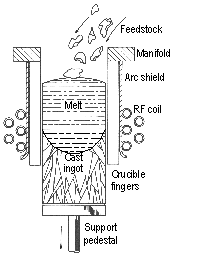
\includegraphics[width=3.0in]{EMcasting.png}
        \captionof{figure}{Directional Solidification}
        \label{fig:DS}
 \end{minipage}
 
DS process is achieved by a uni-directional extraction of heat from the melt which leads to a planer movement of solid-liquid interface. As shown in Figure\ref{fig:DS}, MGS is provided as feedstock for DS and converted into molten silicon. Heat is then extracted from the bottom surface only, while the other surfaces are insulated to ensure a planer solidification front. The use of DS has an additional advantage in that it will further purify the feedstock through a process known as segregation.

Segregation is the phenomenon of separating a constituent from the forming solid phase via rejection into the melt. The amount of segregation is measured by the segregation coefficient, $k_{0}$
  \[k_{0}=\frac{C_{S}}{C_{L}} \]
where, $C_{S}$ and $C_{L}$ are the constituents' concentration in the solid and liquid phases, respectively. For most metals constituents in silicon, $k_{0}<1$ which means the impurity prefers to stay in the liquid. As solidification within an ingot reaches completion, the impurities concentrate at the top as it is the last part to solidify. This process be be repeated several times to further segregate and remove impurities. The part left behind once the impure part has been removed is used as SGS feedstock for wafer fabrication.  

The rate of cooling is an important parameter during DS. As a slow cooling rate lead to large grain sizes and thus less grain boundary area, it is preferred over a faster cooling. But a slow cooling rate also comes at increased manufacturing time and cost. The rate of cooling during DS also determines the level and the distribution of dislocations formed inside the solid \cite{moller2005multicrystalline, ryningen2011growth}. A faster cooling rate leads to a higher dislocation density due to strain from differential thermal expansion between top and bottom of the ingot. The rate of cooling is therefore a very crucial factor during DS process.

\section{Wafer production by Wire sawing}
SGS ingots from the DS process are converted into solar wafers via sawing techniques. Among the many sawing techniques, multi wire sawing is the most efficient since it can be used to cut all of the ingot at once. 80\% of the SGS wafers produced industrially use multi wire sawing \cite{}. During wire sawing, SGS ingots are glued to a substrate holder and placed in a wire saw which then slices them into thin wafers. This process is shown in Figure \ref{fig:wire-saw}. As can be seen, a single wire is fed from a supply spool through a pulley and tension control unit to four wire guides. The SGS ingot on the holder is pushed down the wire web which leads to material removal and slicing. This wire is under tension during this process, and may be at different levels of strain depending on the depth of the cut.  
\begin{figure}[ht]
    \centering
    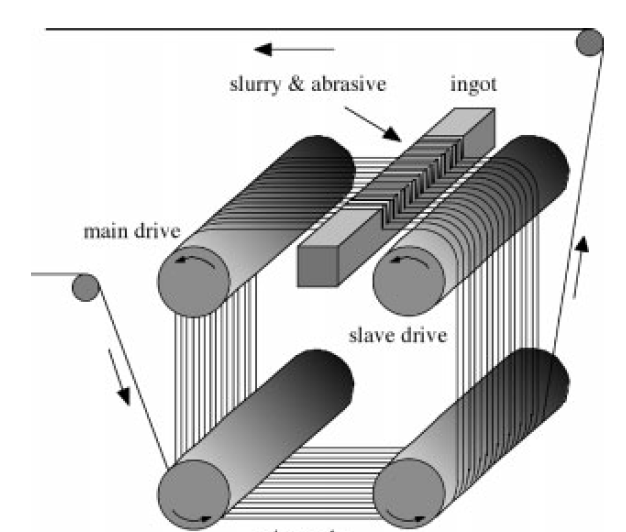
\includegraphics[width=3.0in]{wire-saw.PNG}
    \caption{figure}{Wire Sawing Setup}
    \label{fig:wire-saw}
\end{figure}
The wire is made of stainless steel and has a typical diameter of around 150-200 micron. The volume between the wire and the ingot surface is covered with slurry containing abrasives such as SiC and diamond particles. The size of these abrasive particles are around 5-30 micron \cite{}. The slurry moves with the movement of the wire and acts as a transport medium for the abrasives into the sawing channels. The slurry has to be highly viscous and so usually made out of oil or ethyl alcohol. The slurry also must minimize temperature rise during wire sawing by continually removing the heat of cutting. The actual material removed, also known as Kerf loss, is around 200-250 microns per wafer. Thus, the kerf loss is nearly 50\% of total wafer material. This wastage of material makes wire sawing an expensive method.
\newline
\noindent
\begin{minipage}[c]{\textwidth}
\centering
        \captionsetup{type=figure}
        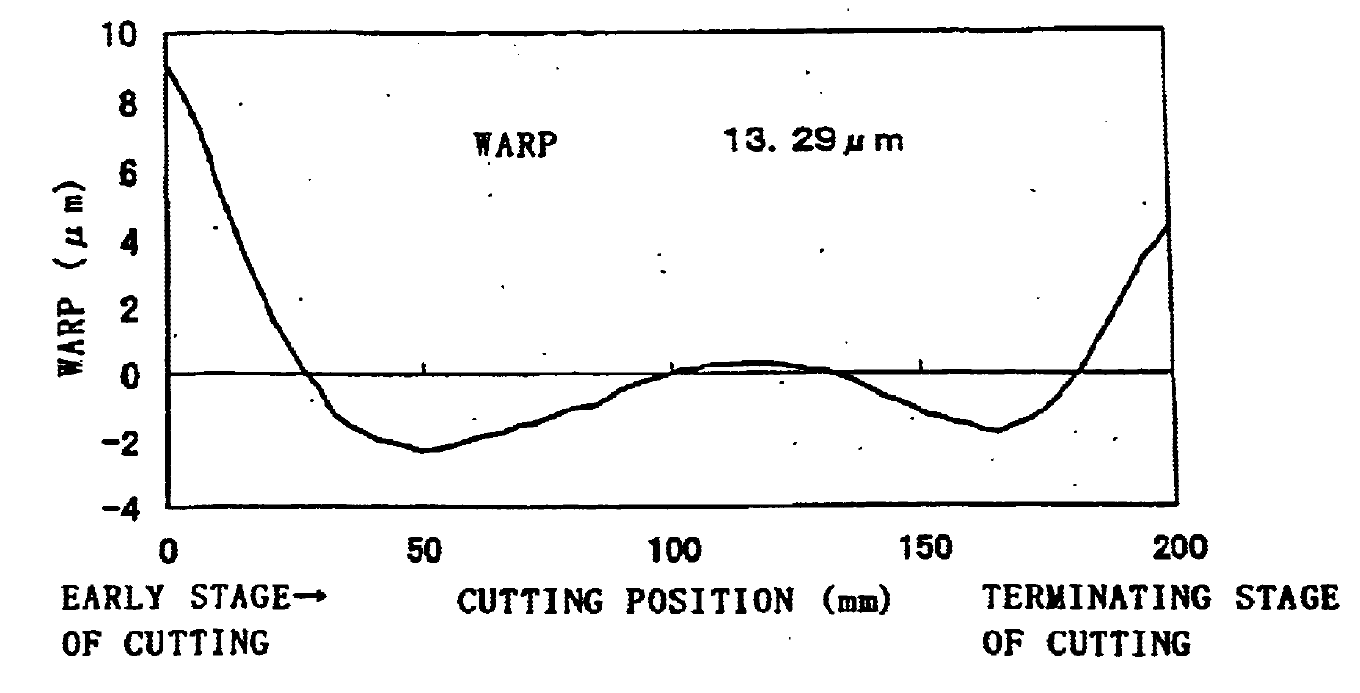
\includegraphics[width=5.0in]{observed-warpage.PNG}
        \captionof{figure}{Warpage in wafers \cite{}}
        \label{fig:warpage}
 \end{minipage}
 
Although wire sawing is an efficient process, the wafer produced can be non flat i.e. have warpage in it as shown in Figure \ref{fig:warpage}. This occurs due the development of thermal gradients between different locations in the work piece during sawing. The amount of warpage depends upon the wire sawing parameters such as wire speed, tension etc and the work piece properties such as residual stress. Warpage in wafers is undesirable as it creates a difficulty during fabrication of solar cells, and reduced photovoltaic efficiency. 

\section{Summary}
Wafers for solar cells are made from SGS material through a multi step process involving DS of mc-Si ingots and wire sawing of these ingots. During these processes, defects such as warpage, dislocations, and residual stresses can be induced in the final wafer which increases component costs and reduces the efficiency of the solar cells. In this thesis, a mathematical model for simulating the dislocation density, residual stress and warpage during processing is developed that can be used to understand the link between processing and solar cell wafer performance. In the next chapter, prior research conducted in the area of numerical simulation of directional solidification and wire sawing, along with the theories developed for predicting the thermoplastic behaviour of silicon are reviewed.
%======================================================================
\chapter{Literature Review}
%======================================================================
\section{Introduction}
Thermo-mechanical simulation of the multi-crystalline Si wafer fabrication process via directionally solidified MGS ingots is a complex problem due to the large number of process parameters involved and the complex properties of silicon. To perform such a task, sufficient knowledge is required of the mechanical properties of silicon, the directional solidification process, the wire sawing process, and finite element modelling. In this chapter, prior literature on these topics is reviewed. The literature can be divided into three distinct areas: (i) constitutive behaviour of Si, (ii) analytical and numerical studies of the directional solidification process, and (iii) analytical and numerical studies of the wire sawing process. 

Experimental studies can be very informative in studying the evolution of dislocations and residual stresses during thermo-mechanical processing. However, experiments involving directional solidification and wire sawing processes require considerable time and costs, so computational models have been developed to simulate the stress and the temperature fields under various cooling rates and material geometries. These models were developed using numerical techniques such as finite element methods and require the mathematical equations behind the the physical processes. The validity of these models, however, needs to be tested against some experimental data. These models can be very helpful to an industrial practitioners who wishes to improve the quality of the products.

\section{Silicon: Properties}
\subsection{Crystal structure and phases}
Si is a covalently bonded material that exists as diamond cubic structure with a face-centered Bravais lattice and a two atom basis. Its lattice parameter is approximately found to be a~0.543 nm at 293 K \cite{hull1999properties}. Si displays allotropy, existing in different phases with a different lattice structures depending on the temperature and pressure. Thermo-mechanical processing of Si leads to phase transformation due to changes in temperature and pressure. This transformation may change the material from ductile to brittle thereby causing failure while during�� processing. At room temperature and 1 bar pressure, Si exists as diamond cubic form Si-I. Indentations and cracks can lead to high stress concentrations and hydrostatic stresses, which can lead to its phase transformation.  Kailer \textit{et al} \cite{kailer1997phase} showed that the cubic Si-I transforms to metallic Si-II at a depth of 0.5 microns under a diamond indenter. This then transforms into amorphous Si at fast unloading rates or a mix of Si-III and Si-XII at slow unloading rates. The area away from the indenter has lower stresses and thus forms Si-IV, which undergoes plastic deformation using the classical dislocation glide and twinning mechanism. Zhang \cite{zhang2004plasticity} has reviewed the different modes of plastic behaviour for surfaces. These modes are summarized in Fig. \ref{fig:phase_trans}. Si undergoes a multi-phase reversible or irreversible transformation depending upon the level of both hydrostatic and deviatoric stresses and loading-unloading conditions. 

\noindent
\begin{minipage}[c]{\textwidth}
\centering
        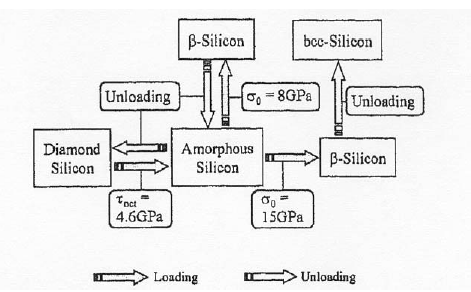
\includegraphics[width=3.0in]{phase-trans.png}
        \captionof{figure}{Phase transformation on Si under stress}
        \label{fig:phase_trans}
 \end{minipage}

\noindent
\begin{minipage}[c]{\textwidth}
\centering
        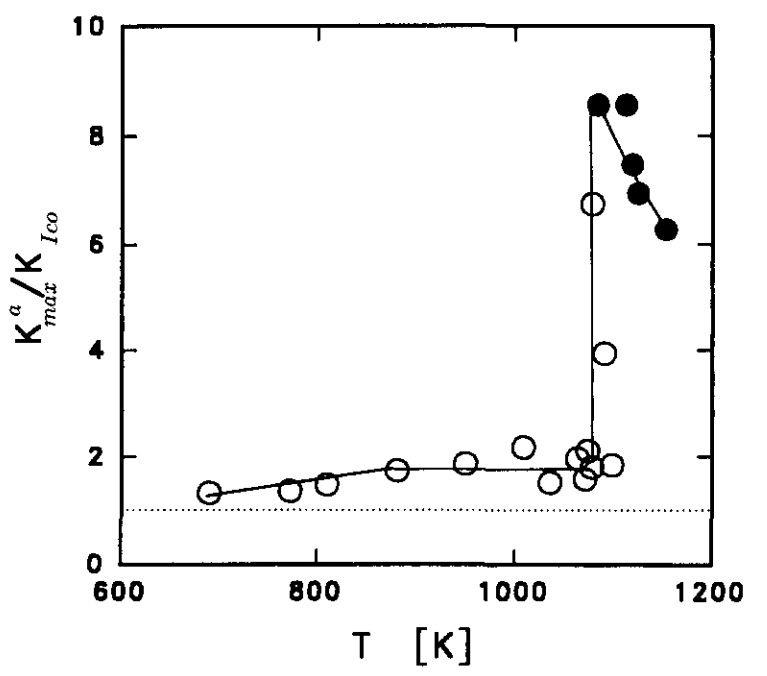
\includegraphics[width=3.0in]{BDT.PNG}
        \captionof{figure}{Brtile to ductile transition of diamond silicon}
        \label{fig:bdt}
 \end{minipage}

Diamond Si has a very high ductile to brittle transition temperature (DBTT); it is brittle at temperatures from ambient to approx. 1000\degree C \cite{brede1993brittle}. It has, however, been also observed that silicon exhibits a ductile behaviour even while processing in brittle regime \cite{liu2007mechanism} under high compressive and sheer stress.
\newline

\subsection{Stress Strain Behaviour}
%\subsubsection{Stress-Strain Behaviour}
Deformation tests have been done \cite{patel1963macroscopic,alexander1969dislocations} to understand the plastic deformation of silicon and germanium crystal at various temperatures and strain rates. These crystals are Float-zone grown and impurity free. These tests are done to understand the different stages of stress-strain curve of silicon. A typically observbed stress-strain curve of a single crystal germanium is shown in Figure \ref{fig:stress-strain}. In the first stage, single crystal exhibits a bell shape stress-strain curve when the strain is less than 2\% of resolved shear strain \cite{patel1963macroscopic}. After stage I, it undergoes two hardening stages, II \& IV and two dynamic recovery stages, III \& V. The inflection in the curve differentiates the various stages.
\noindent
\begin{minipage}[c]{\textwidth}
\centering
       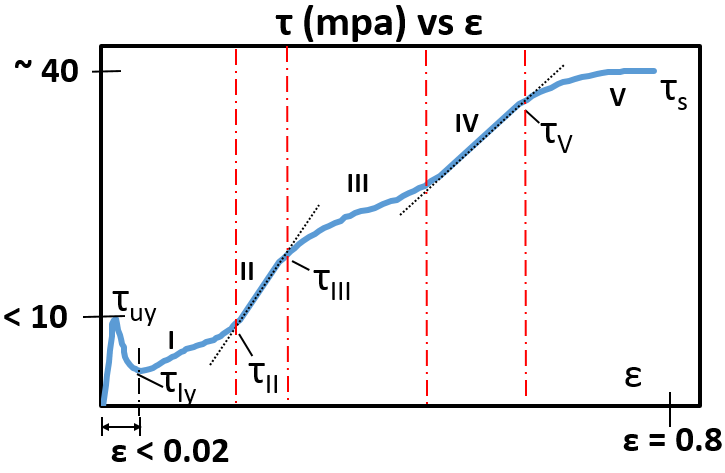
\includegraphics[width=4.0in]{silicon_stress_strain_curve2.PNG}
      \captionof{figure}{Stress-strain curves of germanium monocrystals deformed in tension at different crystallographic orientations at T = 788K and strain rate $\dot{\epsilon} = 2 \times 10^{-3}s^{-1}$}.
        \label{fig:stress-strain}
\end{minipage}

After solidification, the crystal undergoes stage I deformation in which the initial elastic deformation increases the flow stress rapidly till it reaches upper yield stress (UYS), followed by which there is a sharp drop of the flow stress until it reaches the lower yield stress to gradually rise again. The UYS and LYS is dependent on temperature, strain rate and initial dislocation density affect the UYS and the LYS \cite{alexander1969dislocations, yonenaga1978dislocation} as shown:
\begin{equation}
   \tau_{yp} = C_{yp} \dot{\gamma}^{\frac{1}{n_{yp}}} e^{\frac{U_{yp}}{K_{b}T}}
   \label{yield_change}
\end{equation}

Where $C_{yp}$ is a constant with respect to temperature and strain rate, nyp and Uyp are yield point specific parameters and found to be in between 0.45 and 0.8 Tm temperature range [Alexander 1968].
\[U_{uyp} = 1.1, n_{uyp} = 2.1\]
\[U_{lyp} = 0.8, n_{lyp} = 2.9\] 

The variation of UYS with temperature is shown in Figure \ref{fig:stress-temp}. At room temperature the UYS is very high compared to at higher temperature. 

\noindent
\begin{minipage}[c]{\textwidth}
\centering
       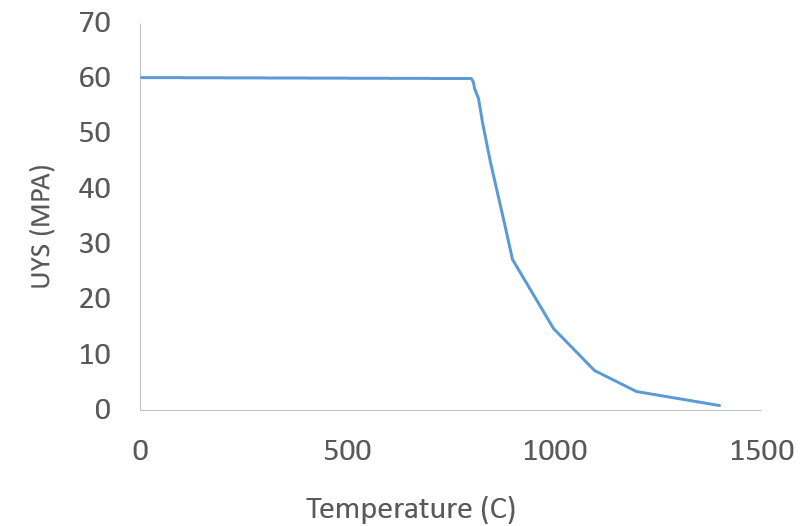
\includegraphics[width=4.0in]{silicon_stress_temp_curve2.PNG}
      \captionof{figure}{Flow stress vs. temperature in silicon for a strain rate of $1.2\times10^{−4} s^{−1}$  \cite{siethoff2001deformation}}.
        \label{fig:stress-temp}
\end{minipage}

\subsection{Dislocation plasticity}

The yield drop is to be due to rapid multiplication of dislocations at UYS. The movement and multiplication of dislocation or dislocation kinetics affects the constitutive behavior of silicon in stage I and so has been reviewed by several researchers the most common of which is given by Alexander-Haasen-Sumino equation written as:
\begin{equation}
   \frac{d\rho_{m}}{dt} = K \rho_{m} v\label{has_1}
\end{equation}
where, $K$ is a function characterizing the dislocation multiplication rate, $v$ is the velocity of the dislocations and $\rho_{m}$ is the change in dislocation density.

A dislocation plasticity constitutive behavior of a material can be used to calculate the dislocation growth and residual stress during application of load while the thermo-mechanical processing. In any such process, the total strain under application of stress can be split into elastic and plastic components. Considering small deformations, the rate of change of stress can be written as :

\begin{equation}
   \dot{\tau} = \mu^{*}\dot{\gamma}_{e} = \mu^{*}(\dot{\gamma}- \dot{\gamma}_{p})\label{rate_eqn}
\end{equation}

Where, $\mu^{*}$ is the effective shear modulus or stiffness. This law is at the macroscopic level, it does not considers the distribution and the velocity of dislocation. In order to connect this macroscopic strain rate with the dislocation kinetics, Orowan law which establishes a relation between inelastic deformation rate and the movement of dislocations, given as:
\begin{equation}
   \dot{\gamma_{p}} = b \rho_{m} \bar{v} \label{orowan_law}
\end{equation}

where, $\bar{v}$ is the overall mean velocity of total dislocations $\rho_{m}$ written as:
\begin{equation}
   \bar{v} = v_{0} \tau_{eff}^{p} exp(-Q/K_{b}T)  \label{mean_velocity}
\end{equation}
\begin{equation}
   \tau_{eff} = \tau -  D\sqrt{\rho_{m}} \label{has-creep}
\end{equation}
Where, $D$ is material constant.
Where, $K_{b}$ is Boltzmann constant, $T$ is the temperature and $k_{0}$ and $Q$ are constants whose magnitudes have been, respectively, found to be approximately $1 \times10^{4}$ - $3.5 \times 10^{4} m/MPA/ sec$ and $2.20 - 2.35 eV$ \cite{imai1983situ}. $\tau_{eff}$ can be considered as the stress necessary to overcome the resistive stress $\tau_{c}$ and move dislocations at any given strain rate. $\tau_{c}$ is a function of several resistive stresses due various interactions such dislocation-impurity interaction $\tau_{DI}$, dislocation-dislocation interaction $\tau_{DD}$, etc \cite{sumino1983interaction} and can be written as: 
\begin{equation}
   \tau_{c} = \tau_{DI} + \tau_{DD} + ...\label{tau_c}
\end{equation}


\section{Modelling of Directional Solidification of Mc-Si}

\subsubsection{dan and steve}
\subsubsection{hamdi}
\subsubsection{nakano}
\subsubsection{takashi}
\subsubsection{cochard}

%During directional solidification, due to the presence of thermal gradient, differential thermal contraction occurs which leads to a stress buildup whose magnitude depends upon the geometry of the material, the rate of cooling and the thermal \& the mechanical boundary conditions. As discussed in the previous section, the dislocation density is a function of overall stress, therefore several finite element numerical simulations \cite{addLater,addlater} have been developed to predict the dislocation density under various cooling conditions during directional solidification.

Simulation of any thermo-mechanical process, such as directional solidification and wire sawing, requires a constitutive behaviour to obtain the temperature dependent stress fields. Since the goal of this work is to simulate warpage and residual stress in wafers as-cut from directionally solidified mc-Si ingots via wire sawing, it is important to review various creep based models developed for these two processes. Many creep based finite element models were found to have been developed for mc-Si directional solidification, however, no creep based model developed for wire sawing were found. So in this section, creep based models for directional solidification are discussed, which will be used in developing a finite element model for both directional solidification and wire sawing in this study.  

There creep based inelastic deformation comes due to rise in dislocation density as discussed in the previous section. Dislocation density distribution during directional solidification of mc-Si can be attributed to stress increase during the cooling of ingot after solidification. There are two classes of theories that explain this dislocation distribution:
\newline
1. Dislocations density rises when the Von Mises stress increases beyond the critical stress required for slipping \cite{alexander1969dislocations}. Thermal gradient along the cooling direction leads to different levels of stresses at different locations in the ingot. An initial homogeneous dislocation density coupled with varying level of stress leads to a distribution of dislocation density \cite{meese2006thermo,nakano2011numerical}. 
\newline
2. Dislocations clusters are nucleated during the crystal growth phase preferentially along grain boundaries and surface, which then propagate in the bulk as the crystal grows. This means that controlling grain orientation through seed may reduce the generation of dislocations \cite{takahashi2010generation}. 

\newline
The two theories suggest different mechanism of dislocation origin and thus require different modelling techniques. In the current work, the first school of idea is considered and, therefore, the literature review covers work done involving finite element numerical simulations developed to predict the dislocation density under various cooling conditions during directional solidification.

In case of any thermo-mechanical process, total strain is a sum of various strains such as elastic, plastic, thermal, dislocation creep etc. This can be written as:
\begin{equation}
\epsilon_{s} = \epsilon_{el} + \epsilon_{pl} + \epsilon_{thermal} + \epsilon_{creep}
\label {strainEq}
\end{equation}

The various models for dislocation simulation during directional solidification of mc-Si ingots developed by various researchers \cite{takahashi2010generation,nakano2011numerical,meese2006thermo} vary on the creep law they consider. The most basic creep laws that can be consider is a the power law creep.

\subsubsection{Power-Law Creep }
Widner and Rehwald widmer1986thermoplastic observed that silicon becomes a viscous material at high temperature and its flow stress depends on both temperature and strain rate which is given as:
\begin{equation}
\sigma_{s} = \sigma_{0} \exp \left ( \frac{-\triangle E}{k_{b} T} \right ) \left ( \frac{\dot{\epsilon}}{\dot{\epsilon}_{0}} \right ) ^{1/n}
\label {power-creep}
\end{equation}
Where, $\sigma$ is the Mises stress in Pa, $\dot{\epsilon}$, the strain rate, $\dot{\epsilon}_{0}$, a reference strain rate equal to $10^{-3} s^{-1}$, $\triangle E = k T_{0}$, the activation energy for the movement of dislocation, and $k_{b}$ is the Boltzman's constant, and T is the temperature in degrees K, $\sigma_{0}$, $\traingle E$, and $n$ are the material-dependent properties. Different values of these variables are proposed by various researchers \cite{patel1963macroscopic,siethoff1968lattice,yonenaga1978dislocation} through experiments.

This thermoplastic constitutive behavior was used to model the creep behaviour and predict the residual stress and the deformations after the directional solidification of mc-Si ingot by M'Hamdi \textit{et al} \cite{meese2006thermo}. This creep law, however, does not predicts the final dislocation density distribution. To do so, a dislocation creep law is used which links the density of dislocation and flow stress. 

\subsubsection{Dislocation Creep Law}

Residual stress simulation of directional solidification of mc-Si ingot using dislocation creep constitutive behavior employ the dislocation kinetics discussed in Equation 2.8 - 2.10. As discussed in Equation \ref{tau_eff}, the dislocations move when stress increases beyond a critical level. The critical stress however is different for different slip planes \cite{miyazaki2007dislocation} and, hence, Equation \ref{tau_eff} can be further expanded as:  
\begin{equation}
\tau^{(n)}_{eff} =  \left | \sigma^{(n)}_{RS} \right | - \tau^{(n)}_{c}
\label {cr-slip}
\end{equation}
where, $\tau^{(n)}_{eff}$ and $\tau^{(n)}_{c}$ are, respectively, the effective and the critical stress on any slip plane $n$ and $\sigma^{(n)}_{RS}$ is the stress in global coordinate system resolved at any slip plane $n$ and the criteria for slip and the movement of dislocation on any slip plane $n$ is:
\[ \tau^{(n)}_{eff} > 0 \] 

A number of studies \cite{sumino1999deformation,franciosi1982multislip,cochard2013novel} have been done to identify the value of $\tau_{c}$ in Equation \ref{cr-slip}. The value of $\tau_{c}$ can depend on several factors, as discussed in the previous section, such as dislocation-dislocation interaction, dislocation-impurity interaction, dislocation-grain boundary interaction. 
These factors in formulating $\tau_{critical}$ are discussed below:
\newline
1. Dislocation-Dislocation interaction affects the value of $\tau_{c}$ as it creates a back stress $\tau_{b}$ on the movement of dislocation. A dislocation may be trapped and become immobile and don't contribute to inelastic flow. Total dislocations on a slip plane can be split into mobile and immobile density as:
\begin{equation}
\rho ^{(\alpha)}_{t} = \rho ^{(\alpha)}_{m} + \rho ^{(\alpha)}_{im}
\label {d-d-i}
\end{equation}
The back stress on dislocation movement is developed from inter and intra slip-plane interaction with mobile and immobile dislocation \cite{cochard2013novel}. This can be written as: 
\begin{equation}
\tau^{(n)}_{b} = \mu b \sum_{\beta = 1}^{12} \left ( A_{\alpha \beta} \sqrt{\rho ^{(\beta)}_{m}} + 
                                                        B_{\alpha \beta} \sqrt{\rho ^{(\beta)}_{im}} \right )
\label {d-d-i2}
\end{equation}
Where, $A_{\alpha \beta}$ and $B_{\alpha \beta}$ are the coefficients of interaction between dislocation on slip plane $\alpha$ with dislocation on slip plane $\beta$ of type mobile and immobile respectively. However, Franciosi and Zaoui \cite{franciosi1982multislip} have mentioned that back stress resulting from dislocation interactions of several slip planes are not additive, shown below as:
\begin{equation}
\tau^{(n)}_{b} = \mu b \sqrt{\sum_{\beta = 1}^{12} a_{\alpha \beta} \rho ^{(\beta)}_{t}}
\label {d-d-i3}
\end{equation}
Where, $a_{\alpha \beta}$ depend on the type of interaction between the dislocation of slip planes $\alpha$ and $\beta$.
\newline
\newline
$2.$ Oxygen can diffuse inside the bulk during solidification and lock dislocations \cite{sumino1983interaction}. This type of interaction also contributes towards the critical stress required to move dislocations. The dissolved oxygen with a concentration $c_{0}$ applies an internal stress given as:
\begin{equation}
\tau_{0} = f(T) c_{0}
\label {d-d-i4}
\end{equation}
Where, $f(T)$ is temperature-dependent factor which varies linearly with temperature $T$.

The most commonly used dislocation creep equation is known as Haasen-Sumino-Alexander (HAS) creep model \cite{miyazaki2007dislocation,haasen1962plastischen} termed after the people who formulated it. $\tau_{eff}$ as per HAS equation is given as:
\begin{equation}
   \tau_{eff} = \tau -  D\sqrt{\rho_{m}} \label{has-creep}
\end{equation}
Where, $D$ is material constant. The HAS creep equation only considers dislocation-dislocation interaction as the factor contributing towards the critical stress. This equation has been widely used by several researchers \cite{} to model the dislocation growth during directional solidification of mc-Si ingots.

Most of the computational models for dislocation generation and movement in mc-Si during directional solidification \cite{} take a J2 plasticity isotropic approach and consider only 1 slip plane to simplify the simulations. Some however \cite{} have taken a crystal plasticity approach to simulate dislocation growth on various slip planes. The second approach has been found to be more accurate \cite{} and more insightful for cases which have anisotropic property due to selective crystal orientation of grain.  For this study, a J2 based isotropic approach is considered. This is because a crystal plasticity approach requires experimental data on grain orientation in form of an EBSD micro-structure \cite{CPFEM} which was not available for this work. 


\section{Wire Sawing}
This section reviews the physics of wire sawing process and the effects of various processing factors during wire sawing on the quality of the wafers. Some of these processing factors and the parameters affecting them are summarised as following:
\begin{itemize}
\item
Wire - Tension, Velocity, Diameter, Vibration
\item
Slurry - Viscosity, Heat Transfer Coefficient
\item
Abrasives - Density, Shape, Size.
\item
Ingot - Residual Stress, Dislocations, Anisotropy
\end{itemize}


These factors affect the final wafer quality in terms of flatness, residual stress and fracture strength. The next section, therefore, discusses the various investigations done regarding some of the underlying physical process that happen during wire sawing and how the wire sawing parameters affect the properties of the wafers.

\subsection{Wire Sawing Models}
Wire sawing is a complex process. As discussed in section 1.4, it involves cutting of silicon ingot by abrasive particles moving with the movement of slurry due to the torque provided by the rotation of wire. The temperature gradient between various locations in the workpiece during this process could be around 40-80 degree C \cite{} which may lead to differential expansion and residual stress causing bending or breaking of wafers. Furthermore, the maximum temperature during wiresawing could reach to around 800 degree C \cite{}, and at this temperature regime silicon undergoes thermoplastic creep deformation which may lead to warpage. Silicon is however, a brittle material around the room temperature, and undergoes cutting due to propagation of cracks developed by the indentation of abrasives on the work-piece and therefore analytical models to study material removal and crack development have been developed using fracture mechanics and indentation theory \cite{}.

In order to calculate the warpage in the wafer during wire sawing, the current work focuses only on the stress buildup and the deformations developed in the work-piece during wire sawing. This involves identifying the temperature rise and the rate at which the material is removed in the work-piece under various wire sawing parameters. So the reviewed literature covers two major aspects: temperature rise and  material removal rate. Temperature rise covers experimental \cite{citation from bhagwat} as well as analytical \cite{swis guy} and numerical \cite{bhagwat} models to measure temperature rise during wire sawing. Material removal rate covers the quantitative models developed to determine the rate at which material is removed with the movement of wire depending on the abrasive particle density in the slurry, the wire tension and the contact span length. 



\subsubsection{Temperature Rise}
Ariga \textit{et al}  \cite{ariga2003wire} and Lundth \textit{et al} \cite{} have measured the final temperature variation across the wafers after wire sawing to be around 20 degree. Bhagavat and kao \cite{} have developed an analytical model and used this to numerically simulate the temperature rise during wire sawing \cite{}. The heat flux entering into the work-piece from the wire and the natural convection through the new surface formed was applied by them to generate this temperature profile. They have also suggested an intelligent control of boundary conditions which can reduce the warpage in wafers by changing the ambient temperature such that the work piece always stays close to room temperature. They have claimed that the simulated temperature profile in the work-piece from their simulations to be in close agreement with the experimental profile from Ariga \textit{et al} \& Lundth \textit{et al} as shown in Firgure \ref{fig:temp-rise}.
\newline
\noindent
\begin{minipage}[c]{\textwidth}
\centering
        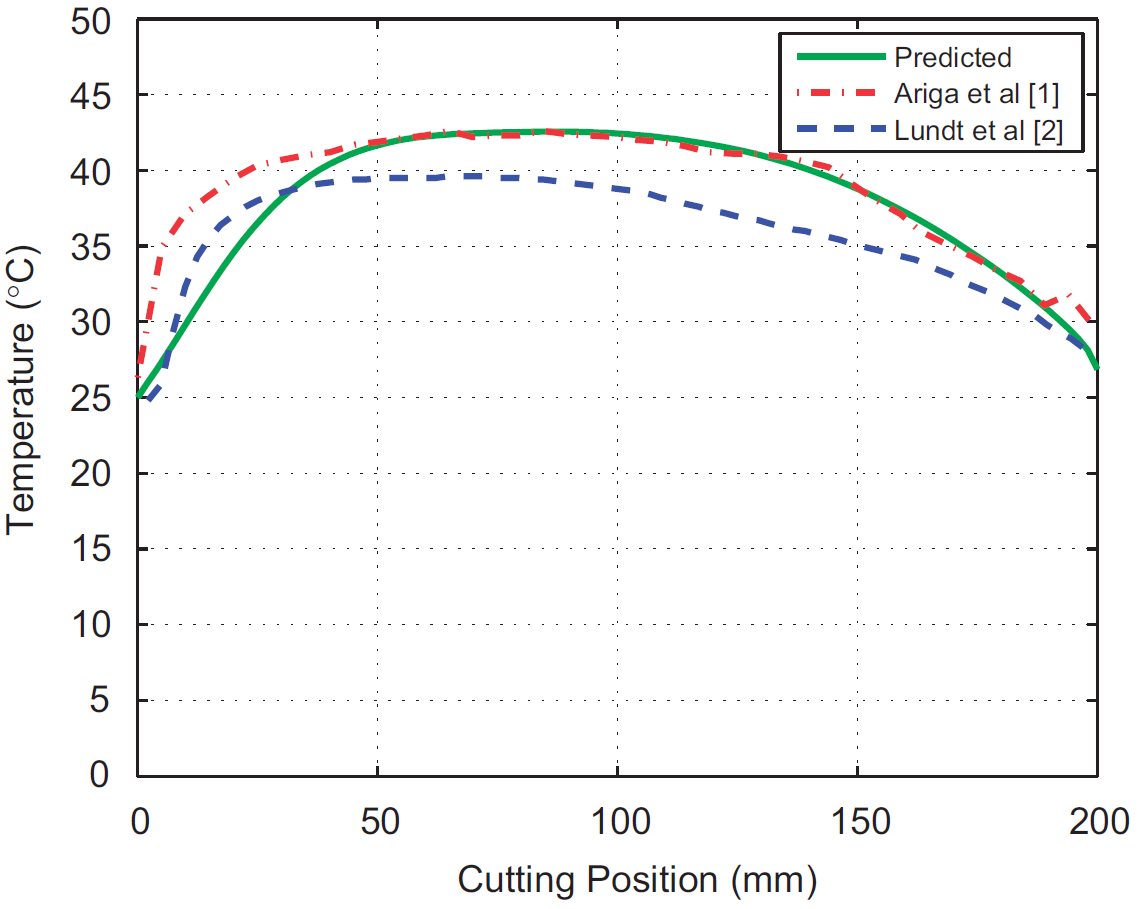
\includegraphics[width=4.0in]{temp-rise-bhagavat.PNG}
        \captionof{figure}{Temperature profile predicted by Bhagavat \& Kao during Wire Sawing}
        \label{fig:temp-rise}
 \end{minipage}

\subsubsection{Material Removal Rate}
Moller el al [ref] have developed several models to relate the material removal with cutting speed and wire load based on the indentation created by particles on the surface of the ingot. The amount of indentation was found out to be dependent mainly upon the frequency of abrasive particles touching Si surface per unit length. Material removal occurs by propagation of the cracks developed from indentation. They further distinguish the cutting process between a non-contact and a semi-contact regime based on the distance between the wire and the ingot surface with respect to the abrasives size. Semi-contact regime is predicted at high stress and low velocities and non-contact regime at low stress and high velocities.

The material removal rate $v_{s}$ as per their model can be written as:

\begin{equation}
v_{s} =  \frac{m \ \ V_{0}}{A_{s} \  \triangle t}
\label {cr-slip}
\end{equation}
\newline
Where, $m$ is the indentation events per unit contact area $A_{s}$ in time $\triangle t$ and $V_{0}$ is the material removed per indentation event. Based on indentation and fracture mechanics, $V_{0}$ has been found to be a function of normal force $F_{N}$ acting on the work piece as:
\begin{equation}
V_{0} = F^{2.2}_{N}
\label {cr-slip}
\end{equation}
\newline
As per these equations, it is clear that the material removal rate is a function of the contact length between the wire and the work piece since with increasing contact length, $A_{s}$ decreases. So for a cylindrical work piece, this result can be used for creating time steps depending upon the depth of cut while creating a numerical simulation for calculating the temperature and the stress fields during wire sawing.


%\subsection{Summary}
%In this chapter, theory of dislocation kinetics in silicon has been discussed first. Followed by this, works on numerical simulation of direction solidification based on the theory of dislocation kinetics has been discussed. Finally theory of wire sawing has been discussed. The various equations used are summarised below
%======================================================================
\chapter{Scope and Objectives}
%======================================================================
\section{Scope of this Research Work}

In recent years, wafers for solar cells are being produced by wire sawing of directionally solidified mc-Si ingots. The wafers produced this way have two issues. 1. Loss of efficiency due to presence of defects such as dislocation, impurity atoms and grain boundary. 2. Warpage due to thermoplastic deformation during wire sawing and the presence of initial residual stress in the work piece i.e. directionally solidified mc-Si ingots.

Over the years, a number of finite element models have been developed for predicting dislocation growth and residual stress during DS process of mc-Si. These models take into account the various dislocation kinetics models of silicon. When it comes to wire sawing, however, there are limited finite element models available for predicting warpage and reisudal stress. For thermal simulation, the only finite element model developed is by Bhagavat and Kao \cite{} and for stress simulation, there are only analytical models derived from the work of Moller et al \cite{}. The goal of this work is do simulate warpage in wafers as-cut from directionally solidified ingots. To perform such simulation a finite element model is developed both for DS process and wire sawing process with the later taking the results of the former as initial conditions.


\section{Objective of this Research Work}
This research work, as shown in Figure \ref{fig:objective}, is done in three steps
\newline
(1). Thermal and stress simulation of DS process.
\newline
(2). Post processing and mapping of the results from above simulations on a wire sawing simulation mesh.
\newline
(3). Thermal and stress simulation of wire sawing process.
\newline
\newline
\noindent
\begin{minipage}[c]{\textwidth}
\centering
        \captionsetup{type=figure}
        \includegraphics[width=4.0in]{flowchart.png}
        \captionof{figure}{Overview of the simulations}
        \label{fig:objective}
 \end{minipage}
 
 \section{Limitations}
 
There are some limitation to this work. In this modelling, effect of grain boundary and impurities are not considered. Also slipping on multiple plane is not considered and an insotopic J2 plasiticity model has been developed. the In wire sawing simulation, fracture mechanics due to interaction between the abrasives \& the ingots and hydrodynamics between slurry and abrasives has not been considered. The fracture strength of wafer based on the surface crack density, also based on Weibull modulus, is not reviewed. The only properties studied in the final wafer is the warpage and the residual stress. 
%======================================================================
\chapter{Model Development}
%======================================================================
\section{Introduction}
In this thesis, the objective is to develop a numerical model to simulate the residual stress and  dislocation density found in Si wafers produced for solar cell applications. The manufacturing process involves casting via directional solidification and then wire sawing. Both process steps involve significant thermal loads and mechanical deformation. In order to determine the material state after wire sawing, it is important to solve the temperature-time and the stress-strain mathematical equations simultaneously. Solving these equations is challenging because they require accurate material properties, boundary conditions, geometry and state equations (for stress and dislocation). These material properties can vary significantly depending upon the purity and grain structure of silicon. The boundary conditions and geometry can vary depending on the physical setup for which the process is being simulated. 

Mathematical equations for any physical process such as temperature evolution and mechanical deformation can be solved using numerical methods. One of the most commonly used numerical methods for solving problems related to continuum mechanics is finite element analysis (FEA). In this research project, the commercial finite element software package ABAQUS 6.12 has been used to model the processing of Si wafers. This software is an efficient explicit/implicit finite element simulation package with excellent capability to solve transient heat transfer problems and mechanical deformation problems, and is very well documented. 

\section{Model Formulation, Domain \& Geometry}


\subsection{Analysis Formulation}

The finite element prediction of the residual stress and dislocation density after directional solidification and wire sawing requires solving the heat transfer and stress-strain partial differential equations. The heat transfer equation during solidification is simplified by neglecting solute convection;  heat conduction is assumed to be the only heat transport medium. The heat transfer equation in the standard form used in the finite element formulation is given by,
\begin{equation}
   \frac{\partial(\rho c_{p} T)}{\partial t} 
   - \nabla\cdot(k\nabla T)
   = \dot{Q}
   \label {heat_eq}
\end{equation}
\newline
where $\rho$ is the density in \SI{}{kg.m^{-3}}, $c_{p}$ is the specific heat in \SI{}{J.kg^{-1}.K^{-1}}, $T$ is the temperature, $k$ is the thermal conductivity in \SI{}{W.m^{-1}.K^{-1}}, and $\dot{Q}$ is the heat generated inside the domain in \SI{}{W. m^{-3}}. In case of solidification model, the term $\dot{Q}$ represents the latent heat. This equation is discretized and then solved to obtain the temperature-time distribution across the domain. 

The main stresses during casting and wire-sawing arise from thermal strains that occur as a result of temperature variations across the domain (if the pressure from the wire is ignored). These thermal strains are then used to calculate the residual stress and dislocation density. The governing equation defining this problem is the equation of motion given by,
\begin{equation}
  \nabla^{}\cdot\sigma_{S} + b
   = 0
   \label {continuity_eq}
\end{equation}
where $\sigma_{S}$ and $b$ represent the stress and the acting body force at any point inside the domain respectively. 

If the strains are small, and deformation is within the elastic regime, then the stress tensor $(\sigma)$ and the strain tensor $(\epsilon)$ have a linear dependence proportional to a stiffness matrix $[D^{el}]$ as per Hooke's law, 
\begin{equation}
  (\sigma)
   = [D^{el}] (\epsilon^{el})
   \label {Hookes_law}
\end{equation}
where the matrix [$D^{el}$] contains the material elastic constants that are a function of elastic modulus and Poisson’s ratio. Beyond the elastic regime, the relation between stress and strain is no longer linear and thus [$D$] depends upon the respective constitutive behavior of the material. In finite element analysis, this is simulated incrementally, i.e.,
\begin{equation}
  d\sigma
   = D^{ep} d\epsilon^{ep}
   \label {Hookes_law_partial}
\end{equation}
where $d\sigma$ and $d\epsilon$ represent the increment of stress and strain, and [$D^{ep}$] represents the inelastic constitutive behaviour of the material.

The ABAQUS software contains four built-in constitutive models: elastic-plastic, elastic-viscoelastic, elastic-creep and elastic-creep-plastic. As discussed in the literature review, the constitutive behaviour of Si during casting and wire-sawing is majorly governed by islocation creep deformation, and so the elastic-creep ABAQUS scheme is used in this thesis. A custom  subroutine has been written in FORTRAN 77 to implement the disllocation creep model. This will be discussed later in the document. 

Within ABAQUS, thermal-mechanical FEA can be performed in one of two ways. First, known as fully-coupled analysis, the heat transfer and stress-strain equations are solved simultaneously. Second, known as sequential coupling analysis, the heat transfer equation is solved first and its results are then applied to the mechanical model when solving the stress-strain equations. The first option is used when the heat transfer and the stress-strain equations have a strong mutual dependence. The second option is used when the interaction can be approximated as one way i.e. the stress-stress equation is dependent on the heat transfer equation.

In finite element methods, the correctness of a solution is determined by how small are the residual values. These residual values are mathematical functions of expected and calculated solution values. In any type of analysis, at each increment, the ABAQUS solver does several iterations till residual $R$ is close to 0 within an error tolerance  $\epsilon$. This is called a convergence criteria,
\begin{equation}
||R||<\epsilon
\label {residualsl}
\end{equation}

Mathematically, the fully coupled analysis can be written as, 
\begin{equation}
\begin{bmatrix}
K_{uu} &  K_{uT} & \\ 
K_{Tu} &  K_{TT} & \\ 
\end{bmatrix} 
\begin{pmatrix}
\nabla u\\ 
\nabla T
\end{pmatrix}
= 
\begin{pmatrix}
R_{u}\\ 
R_{T}
\end{pmatrix}
\label {coupled_anal}
\end{equation}
where $\nabla u$ and $\nabla T$ are the respective corrections to the incremental displacement and temperature, $K_{ij}$ are components of the unsymmetric Jacobian matrix and $R_{i}$ are mechanical and thermal components of the residual vector. ABAQUS solves this coupled system using the Newton-Raphson method with the heat transfer and the strain-strain differential equations solved using backward-difference scheme.

In case of a weak coupling or a sequentially coupled analysis, the off-diagonal submatrices $K_{uT}$ are $K_{Tu}$ are small compared to the components in the diagonals in the Jacobian matrix of Equation \ref{coupled_anal}. The off-diagonal components can be set to 0 as shown,
\begin{equation}
\begin{bmatrix}
K_{uu} &  0 & \\ 
0 &  K_{TT} & \\ 
\end{bmatrix} 
\begin{pmatrix}
\nabla u\\ 
\nabla T
\end{pmatrix}
= 
\begin{pmatrix}
R_{u}\\ 
R_{T}
\end{pmatrix}
   \label {sq_coupled_anal}
\end{equation}
Due to this approximation, the thermal and the mechanical equations can be solved separately and more efficiently, reducing computation time.

The main issue with sequential coupling in this project is the need to take extra precautions while solving the stress-strain equations since the stress fields, which are linked to the generation of dislocations, are very sensitive to temperature changes. Under such temperature-dependent kinematical framework, even a small error in the temperature field might introduce large errors in the stress-strain fields and hence a high level of accuracy in temperature is required. In this work, errors in the temperature are minimized by enforcing a small maximum time steps of 2s in the thermal model. This considerably increased the processing time but ensured accuracy. The overall scheme was implicit.

\subsection{Model Domain, Geometry and Meshing}

\subsubsection{Casting}

The analysis for directional solidification assumed that the mc-Si casting was cylindrical, and was being performed in a Crystalox DX-250 furnace, with dimensions 250mm in diameter and 105mm in height. The goal was to characterize the thermal evolution of the ingot during directional solidification, along with the residual stress and dislocation density states at the end of the casting process. Due to symmetry along the centreline, the finite element analysis is only required for a one-half radial section having dimension of 125mm by 105mm. Further, this approach converted the problem of solving the heat and mechanical equations in 3D into a axi-symmetric, saving computational time. The geometry was meshed with 1548 nodes and 1470 elements with each element having four nodes. The element types used for thermal and stress models were axisymmetric diffusive heat transfer element and axisymmetric reduced-integration solid element given by DCAX4 \& CAX4R respectively in ABAQUS. This mesh is shown in Figure \ref{fig:casting-mesh}.

This objective of this analysis was also to study the residual stress and the dislocation density under slow, medium and fast cooling. This however required the correct value of the convective heat transfer coefficient of the bottom surface via which the heat was escaping from the ingot. Under the lack of this critical information, the cooling was simulated by assuming the bottom surface to cool at 2, 5 and 8 K/Min, mimicking slow, medium and fast colling respectively. The time supplied for simulation was, therefore,  900, 300 \& 200 minutes respectively for slow, medium and fast cooling. The extra time was supplied in the cooling simulations to ensure that all the points in the domain have reached 298 K and there is no final temperature gradient inside the domain. The term residual stress is different from stress and it refers to that stress which is present inside the domain after all type of load has been removed, thermal in this case. This is why it is important that there is no final thermal gradient inside the ingot. 

This cooling scheme is a very lose approximation of the real cooling phenomenon but the way this simulation scheme is developed, a complex heat transfer coefficient can be be fed into this scheme to obtain better results in the future.


\begin{figure}[h]
    \centering
    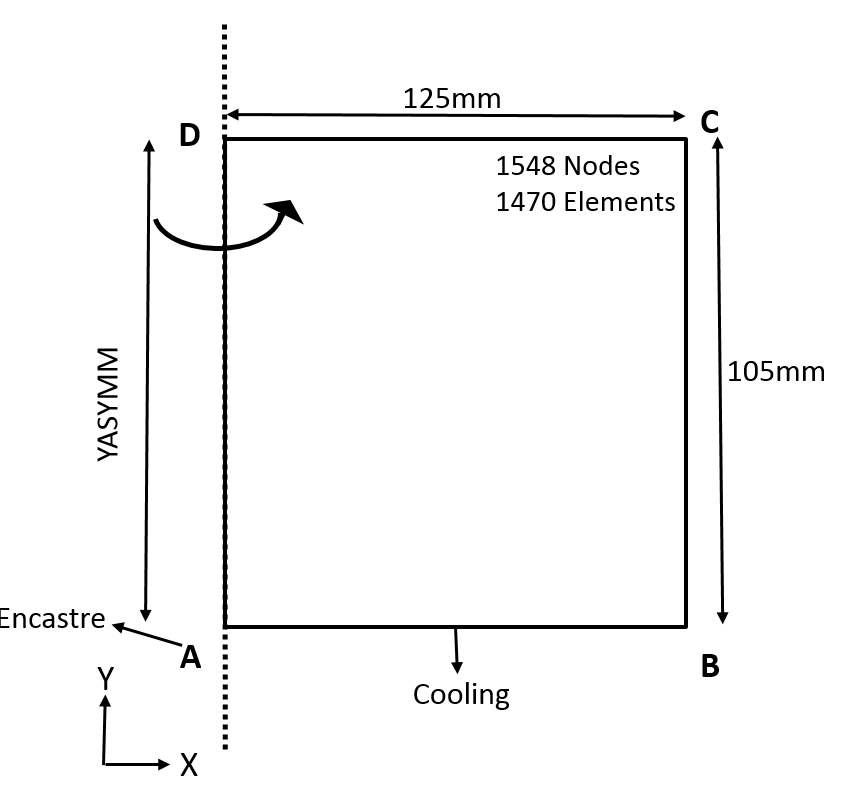
\includegraphics[width=4.0in]{casting-mesh.PNG}
    \caption{Mesh for casting simulation}
    \label{fig:casting-mesh}
\end{figure}

\subsubsection{Wire Sawing}
The aanalysis domain for wire sawing model was a circular volume with diameter 250 \SI{}{mm} and height 1500 \SI{}{\micro.m}. The goal was to determine the amount of warpage and dislocation density in as-cut Si wafers taken from different heights along the ingot. The wire sawing simulations were performed on three different locations within the casting: 26.25, 52.5, and 79.75 \SI{}{mm} from the base of the ingot. The reason for performing the analysis on these sections instead of the whole ingot was to minimize computational cost and time. The caveat of this approach is the need to correctly map stress, strain and dislocation density from the casting model onto these sections. The first step was to map the stress, displacement, and dislocation density fields from the results of the casting simulation as initial conditions. Once mapped, the next steps were to perform the thermal and mechanical simulations. For all the three sections, only a single thermal model was built because it was assumed that the temperature profile while multi-wire sawing does not vary along the axis of the ingot. The mechanical models were built separately for these three sections, and applied the temperature results from the thermal simulation as a pre-existing field. The time for wire sawing was taking as 500 minutes since, industrially, this is the time that it takes for multi-wire sawing of Si ingots.  

An axisymmetric mesh could not be used for modelling wire sawing because it is not a symmetric operation. A special type of mesh, as shown in Figure \ref{fig:wiresawing-mesh}, was constructed by writing a script in PYTHON. This mesh had parallel lines perpendicular to the feed movement direction. This meshing was used to simulate a material removal pattern with wire movement from the entry point to the exit point. Note that, this mesh is still an approximation to wire sawing since in reality the wire bows while slicing. This mesh had 9608 nodes and 6903 elements with 8 nodes per element for both the thermal and stress models. The 3D diffusive heat transfer DC3D8 and continuum C3D8 elements were used for the thermal and mechanical model respectively.

\begin{figure}
    \centering
    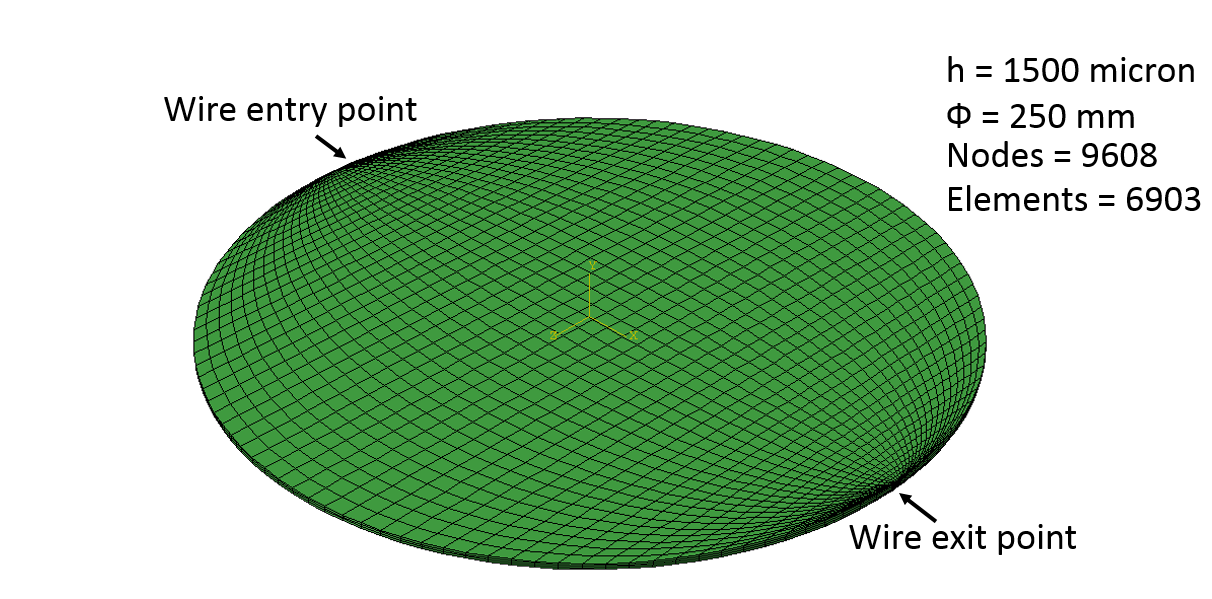
\includegraphics[width=5.0in]{wiresawing-mesh.PNG}
    \caption{figure}{Mesh for wire sawing simulation}
    \label{fig:wiresawing-mesh}
\end{figure}

\section{Input Material Properties}

\subsection{Thermal Properties}
The thermal properties of liquid and solid silicon, required for performing the temperature finite element analysis, include: density, latent heat of fusion, heat capacity, and thermal conductivity. These are tabulated along with their respective sources in \ref{table:thermal-prop-1} and \ref{table:thermal-prop-3}. Impure materials usually solidify over a range called as liquidus-solidus temperature range depending upon the concentration of primary and secondary constituents in it. For a material with high concentration of one constituent, the liquidus-solidus range is small. During directional solidification of mc-Si from MGS, due to the 98\% purity of silicon, this range is between $0.5-1\degree C$ around the melting point temperature i.e. $1410\degree$C. Thermal conductivity of silicon depends on temperature \cite{glassbrenner1964thermal} and changes significantly from room temperature to its melting point.

\begin{table}[h]
    \centering
    \begin{tabular}{|c|c|}
    \hline
    $T_{solidus}$ (\SI{}{K}) & 1682.5 \\ 
    \hline
    $T_{liquidus}$ (\SI{}{K}) & 1683 \\
    \hline
    Latent Heat (\SI{}{kJ.kg^{-1}}) & 1926 \\
    \hline
    \end{tabular}
    \caption{Thermal property of Si \cite{}}
    \label{table:thermal-prop-1}
\end{table}

\begin{table}[]
    \centering
    \begin{tabular}{ |c|c|c|c|}
    \hline
    $T$ (\SI{}{K}) & $k$ (\SI{}{W.m^{-1}.K^{-1}}) & $T$ (\SI{}{K}) & $k$ (\SI{}{W.m^{-1}.K^{-1}})  \\
    \hline
    200 & 266 & 1000 & 31 \\
    \hline
    300 & 156 & 1100 & 28 \\ 
    \hline
    400 & 105 & 1200 & 26 \\
    \hline
    500 & 80 & 1300 & 25 \\ 
    \hline
    600 & 64 & 1400 & 24 \\ 
    \hline
    700 & 52 & 1500 & 23 \\ 
    \hline
    800 & 43 & 1600 & 22 \\ 
    \hline
    900 & 36 & 1681 & 22 \\ 
    \hline
    \end{tabular}
    \caption{Specific heat of Si with Temperature \cite{}}
    \label{table:thermal-prop-3}
\end{table}

Silicon has a unique liquid-solid density change property, unlike other elements, as liquid silicon is denser than solid silicon meaning that solid Si has the potential to float during solidification. However, for this analysis, this material behavior is ignored to reduce complexity. The variation in density with temperature for solid Si is also ignored because adding that feature to the model would change the mass balance of the system.



\subsection{Mechanical Properties}
The mechanical properties required for performing the stress finite element analysis are: density, elastic moduli, Poisson’s ratio, thermal expansion, and dislocation creep behavior. These properties are tabulated in table \ref{table:mech-prop-1}, along with their respective sources.

\begin{table}[]
    \centering
    \begin{tabular}{ |c|c|c|c| } 
    \hline
    Property & Temperature range (K) & Value\\
    \hline
    $\alpha(T)$ (\SI{}{K^{-1}})  & 298$<T<$1683 & 3.725$\times 10^{-6} \cdot [1-e^b]$\\
     & & $b=-5.88 (T-124) 10^{-3}+5.55 T 10^{-4}$\\    
    & 1683 $<T$ & 0  \\
    \hline
    $\rho$ (\SI{}{kg.m^{-3}}) & N/A & 2330 \\
    \hline
    E (\SI{}{G.Pa}) & 298$<T<$ 1683 & $1.7 \times 10^{11} - 2.771 \times 10^{4} \times T^{2}$\\
    & T $=$ 1713 & 100\\
    & T $=$ 1773 & 1\\
    \hline    
    $\nu$ & N/A & 0.22\\    
    \hline 
    \end{tabular}
    \caption{Mechanical property of Si \cite{}}
    \label{table:mech-prop-1}
\end{table}

\subsubsection{Coefficient of thermal expansion:}

If coefficient of thermal expansion is a function of temperature or field variables, then the total thermal expansion coefficients at various temperature is required in tabular format as input in ABAQUS along with the reference temperature as shown in eq \ref{thermalExp}.
\begin{equation}
\alpha(T) = \frac{1}{T-T^{0}}\int_{T^{0}}^{T} {\alpha}'(T)dT
\label {thermalExp}
\end{equation}
where, $\alpha$ is the effective thermal expansion, ${\alpha}'$ is the temperature dependent thermal expansion coefficient and $T^{0}$ is the a reference point specifying the critical temperature where the material can assume zero thermal strain. $T^{0}$ was taken as 1683K since in molten form there is no strain. The total thermal expansion $\alpha$ can be imagined as the average rate of change of length with temperature rather than instantaneous rate of change.  

\subsubsection{Elastic modulus:}

The elastic modulus is a function of temperature changing from 91 GPa at room temperature to 167 GPa at melting point. Above the melting point it is ramped down to a significantly lower value over the next 50 K to give metal the liquid property of flow due to tensile stress.

\subsubsection{Stress – Strain data:}

As shown in SEC X.X, there are a lot of existing literature on stress-strain characteristics of silicon under tension at various temperatures. In this analysis elastic-creep behavior is considered. The inelastic deformation occurs to compensate for the movement and multiplication of dislocation. Rate dependent plastic behavior and yielding are not considered.


\section{Initial \& Boundary Conditions}


\subsection{Casting: Thermal Model}
Thermal initial conditions were specified for the ingot. All the nodes were set to 1773 K, which is the temperature till which silicon is heated in the furnace before the solidification process starts. 
Thermal boundary conditions were placed on all edges of the mesh shown in Figure The edge BC \& CD are assumed to be insulted. Heat is exiting from the ingot by convection through the bottom edge AB. Dirichlet boundary condition is applied to nodes on AB to simulate cooling rates of 2, 5 and 8 K/Min. This was implemented by creating a surface film in ABAQUS to facilitate surface convection. The sink temperature of this film was changed at 2, 5 and 8 K/Min and the film coefficient was assigned a large value so that the nodes at surface AB cool at the same rate as the sink. This cooling boundary condition is applied because in this work there is no experimental cooling curve data and the of value of natural surface convection coefficient $h$ in Equation () is not known. 

\subsection{Casting: Displacement Model}

%\subsubsection{Initial Conditions}
A dislocation density of $10^8$ \SI{}{m^{-2}} is supplied as the initial field condition for all the nodes in the displacement model. Initially there is no elastic or plastic strain is present in the ingot. So no initial stress or strain is applied. Predefined temperature field is supplied using *TEMPERATURE in ABAQUS to read the temperature data from the thermal model. At all the increments the temperature data from the thermal model output database is read and subjected as temperature to calculate the thermal strain.

%\subsubsection{Boundary Conditions}
Mechanical boundary conditions are applied at the nodes on the side DA. All the nodes are constrained to move in Y direction only. The bottom most node is pinned to ensure that the center of the bottom of the ingot is always touching the crucible. All the other nodes are having all degree of freedoms for movement. Since the ingot remains inside the crucible at all times so the nodes on BC should be partially constrained to not move radially outwards. But in this case it is known that silicon contracts during cooling, so mechanical boundary conditions are not supplied on the nodes on BC.

\subsection{Wire Sawing: Thermal Model}

%\subsubsection{Initial Conditions}
Initial temperature of 298 K is applied to all the nodes of the wire sawing mesh because the ingot is initially at room temperature. 

%\subsubsection{Boundary Conditions}

\noindent
\begin{minipage}[c]{\textwidth}
\centering
        \captionsetup{type=figure}
        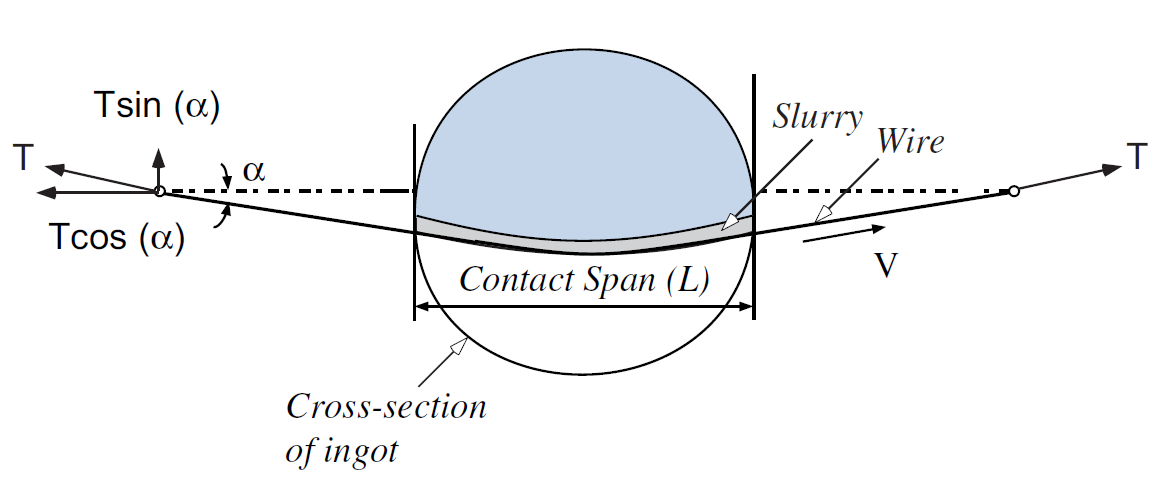
\includegraphics[width=6.0in]{wiresaw-crossection.PNG}
        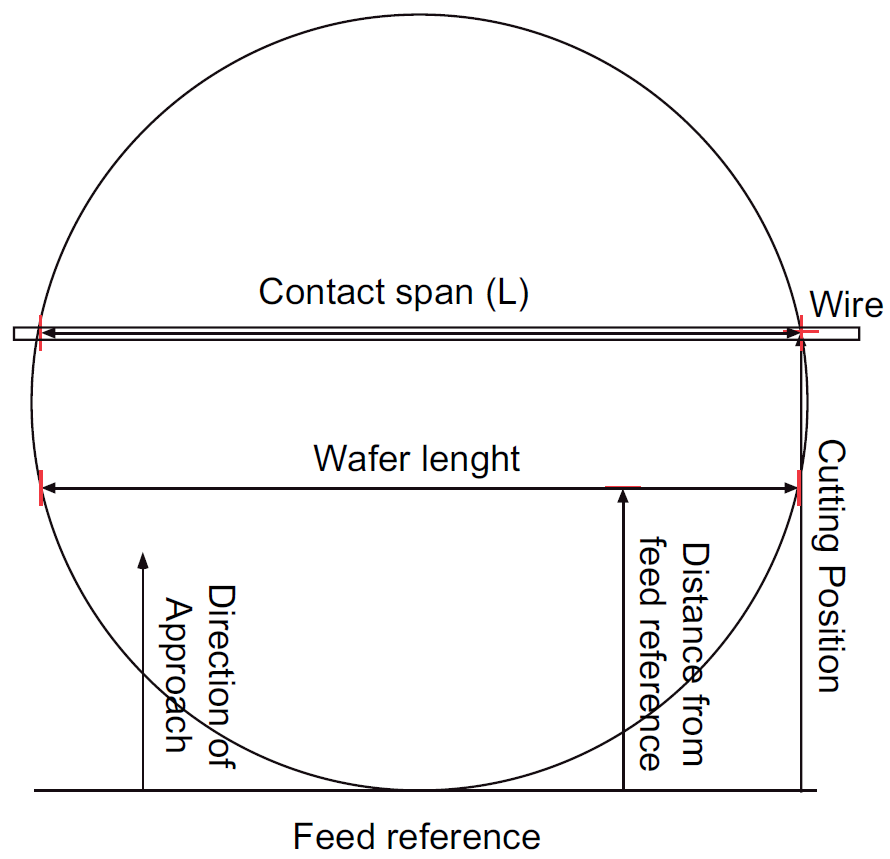
\includegraphics[width=2.5in]{wiresaw-crossection2.PNG}
        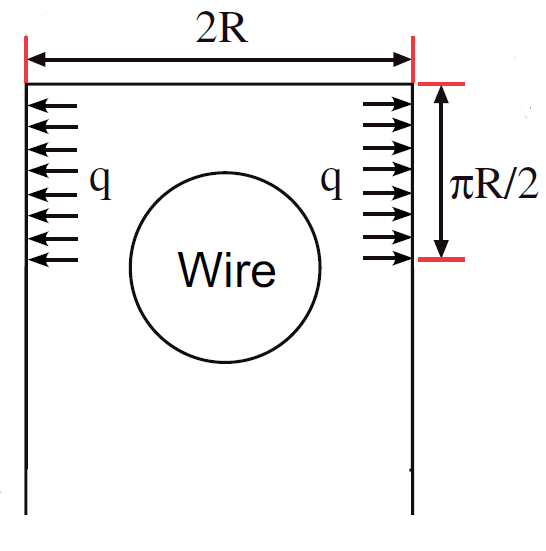
\includegraphics[width=2.5in]{wiresaw-groove.PNG}
        \captionof{figure}{Wire movement}
        \label{fig:wiresawing-crossection}
 \end{minipage}
\subsubsection{Heat Flux}
The most important aspect of thermal modelling of wire-sawing is to the determine the heat flux entering the work piece from the wire and the heat exiting from the new surface formed due to surface convection. Heat flux entering inside the ingot depends upon several factors including wire and slurry parameters. An analytical model has been developed by Bhagwat and Kao [ref] to model this heat flux as a function of power supplied to the wiresaw machine $P$ (\SI{}{W.m^{-2}}), area being machined $A$ (\SI{}{m^{2}}) and a dimensionless quantity $\epsilon$ representing the fraction of power transferred from that is actually being used for slicing.

\begin{equation}
Q = \frac{\epsilon P}{A}
   \label {wire_eq1}
\end{equation}


The power $P$ can be further expressed as 


\begin{equation}
P = Tv
   \label {wire_eq2}
\end{equation}

Where $T$ is the tension set in the wire during slicing, $v$ is the velocity of the wire during sawing. The area being machined can be expressed as

\begin{equation}
A = \pi R L
   \label {wire_eq3}
\end{equation}
Where R is the radius of the groove formed during slicing, L is the contact span. Contact span is the length of wire in contact with the ingot as shown in Figure \ref{fig:wiresawing-crossection}. The dimensionless quantity $\epsilon$ is a function of angle $\alpha$ that it makes with the horizontal axis because of bowing while slicing. The force exerted by the wire can be resolved into horizontal and vertical component. The vertical component of the tension in the is assumed to be responsible for the slicing and can be expressed as $T \sin (\alpha)$. As discussed in Sec. 2.4, the elasto-hydrostatic pressure while wire sawing is a function of contact span length L. Thus, taking these two factors into consideration, the dimensionless constant $\epsilon$ can be defined as 
\begin{equation}
\epsilon = \sin(\alpha) \times L
   \label {wire_eq4}
\end{equation}

$\epsilon$ should also include a constant for the amount of heat dissipating in the slurry. Yamada et al [ref] have estimated that 1/3 to 1/2 of the heat from the wire is taken away by the slurry. However, for this analysis this loss of heat by slurry is ignored for simplicity.  

The flux entering also depends on the length of heat source $l_{s}$ i.e. , as shown in Figure \ref{fig:wiresawing-crossection}, is $\pi R /2 $. During the finite element formulation of this process, however, the flux applied is multiplied with the length of the element $l_{e}$ instead of $l_{s}$. There is an issue in this approach if $l_{e}$ is greater than $l_{s}$ as it supplies extra flux in every step. To balance this, a factor $l_{s}/l_{e}$ is also multiplied to the supplied heat flux. The heat flux increases with cutting depth till the center after which it symmetrically decreases. The increase in flux with the depth of cut till the center is shown in Figure \ref{fig:wiresaw-flux}. 

\noindent
\begin{minipage}[c]{\textwidth}
\centering
        \captionsetup{type=figure}
        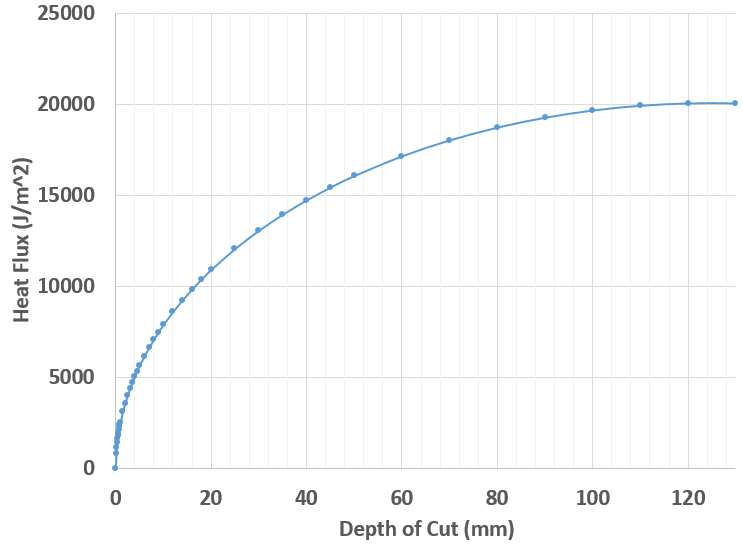
\includegraphics[width=4.0in]{wiresaw-flux.PNG}
        \captionof{figure}{Heat flux with cutting depth}
        \label{fig:wiresaw-flux}
\end{minipage}

\subsubsection{Natural Convection}
During wire sawing simulation, new surface is created at each step of the model. All surfaces that are exposed to the air during slicing, including the newly formed surfaces, are to be applied with natural convection boundary condition. 

Silicon surface has a natural convection coefficient of $h = 5$ \SI{}{W.m^{-2}.K^{-1}} [ref]. But this value can’t be used for the newly formed wafer surfaces. The newly formed wafer surfaces on the work piece is analogous to equally spaced fins, the length which corresponds to the wafer length at a given distance from the feed and height corresponds to the distance from the feed reference. 

The case of natural convection in a Fin has been studied by several researchers [ref-ref]. Harahap and McManus [ref] experimentally found out that convection coefficient decreased rapidly on increase of fin length. Jones and Smith [ref] found out that height of the fin has negligible impact on the convection coefficient of the fin. Chen et al [ref] have analytically solved for convection heat transfer coefficient for a circular annular fin and found it to be a decreasing with decrease in radial distance. For this simulation convection coefficient data is taken from Bhavwat and Kao [ref] which is shown in Figure \ref{fig:wiresaw-h}.  At the cutting position near the feed reference, convection coefficient is 5 \SI{}{W.m^{-2}.K^{-1}} and at the center of ingot it is 0.5 \SI{}{W.m^{-2}.K^{-1}}.

\noindent
\begin{minipage}[c]{\textwidth}
\centering
        \captionsetup{type=figure}
        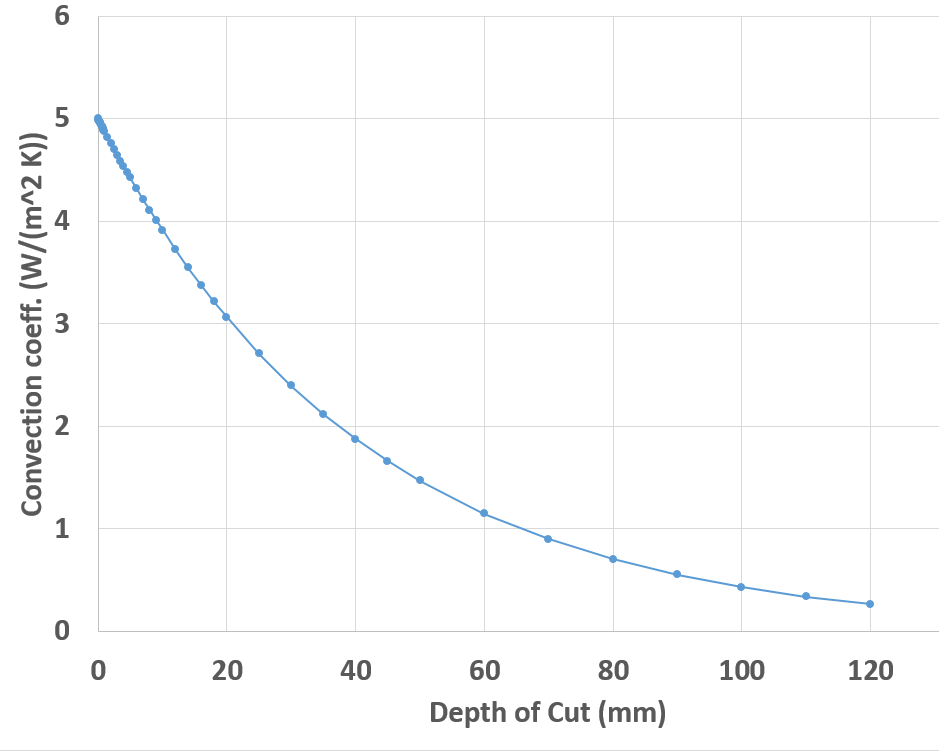
\includegraphics[width=4.0in]{wiresaw-h.PNG}
        \captionof{figure}{Heat flux with cutting depth}
        \label{fig:wiresaw-h}
\end{minipage}

\subsection{Wire Sawing: Displacement Model}

%\subsubsection{Initial Conditions}
Stress, strain and dislocation density results from the casting displacement model are supplied as initial condition for the wire sawing displacement model. Similarly to the casting displacement model, temperature was taken from the wire sawing thermal model at each step using *TEMPERATURE in ABAQUS.  
%\subsubsection{Boundary Conditions}

The mechanical boundary conditions supplied were pinning of nodes at the point where the wire leaves the work piece. This was done because the wafers need to be in fixed contact with some point during the sawing process. 

%Nodes on the surface W1 and W2 where mechanically pinned. This was done because of the way the stress and the strain were mapped from the ingot to the wafer submodel. This will be discussed in more detail while explaining the implementation details of this model in SEC X.X. 


%\input{chapters/chapter_5}
%======================================================================
\chapter{Model Implementation}
%======================================================================
\section{Introduction}

This chapter discusses the methodology of calculating the warpage and the residual stress in the wafers cut via wire sawing from directionally solidified ingots. The methodology comprises of the ABAQUS implementation of the model developed in the previous chapter using the governing equations discussed in the literature review. 

%This chapter discusses the methodology of calculating the warpage and the residual stress in the wafers cut via wire sawing from directionally solidified ingots. The methodology comprises of the governing equations for directional solidification \& wire sawing and the model development. The governing equations have discussed in the literature review and the model development has been discussed in the previous chapter.   

%In this chapter, the finite element implementation of the model developed in the previous chapter is discussed using the governing equations discussed in the literature review section. 

As described in the literature review, several models have been built for simulating residual stress and dislocation density while the DS process of mc-Si ingots using dislocation creep behaviour of silicon. HAS creep model is used in this work to predict the dislocation density developed in silicon under stress. Analytical models for temperature change and material removal rate during wire sawing developed , respectively, by Bhagavat and Moller is used in developing the finite element simulation of wire sawing. The current work consists of three steps: first, simulation of directional solidification, second, mapping the results from above simulation on wire sawing mesh, third, simulation of wire sawing. The mapping was a challenging task since the directional solidification and wire sawing simulation were done on dissimilar meshes. 

The finite element models developed for thermal and simulation for directional solidification and wire sawing are same in terms of governing equations. However, they differ in the initial and boundary conditions along with the meshing and step formulations. While the sequentially coupled thermal-stress simulation of directional solidification is straight forward, the mapping stage and the wire sawing simulation is sophisticated. So their details have been discussed in the later sections.

\section{Governing equations}
The overall strain in a system is the summation of strain contributions from several factors. In the current work, total strain is assumed to be the sum of elastic, plastic, thermal and dislocation creep strain


\begin{equation}
\epsilon_{s} = e^{el} + e^{pl} + e^{thermal} +e^{creep}
\label {strainEq2}
\end{equation}



\begin{comment}

In matrix form, the linear elastic strain for an isotropic material can be written 

\begin{equation} 
\begin{Bmatrix}
 \epsilon_{11}   \\ 
 \epsilon_{22}   \\
 \epsilon_{33}   \\
 \gamma_{12}   \\
 \gamma_{13}   \\
 \gamma_{23}
\end{Bmatrix} = \begin{bmatrix}
 1/E & -v/E & -v/E &  0 &  0 &  0  \\ 
 -v/E & 1/E & -v/E & 0 & 0 & 0  \\ 
 -v/E & -v/E & 1/E &  0 &  0 &  0  \\ 
 0 & 0 & 0 & 1/G & 0 &  0  \\ 
 0 & 0 & 0 & 0 & 1/G & 0  \\ 
 0 & 0 & 0 & 0 & 0 & 1/G  
\end{bmatrix} \begin{Bmatrix}
 \sigma_{11}   \\ 
 \sigma_{22}   \\
 \sigma_{33}   \\
 \sigma_{12}   \\
 \sigma_{13}   \\
 \sigma_{23}
\end{Bmatrix}

\label {strain_matrix}
\end{equation}
\end{comment}

Solving any time varying stress-strain constitutive relation requires knowledge of time varying strain. Time varying linear elastic strain is thus given by
\begin{equation} 
\dot{\epsilon}^{e}_{s} = \frac{1+v}{E}\dot{\sigma}_{s} 
                        - \frac{v}{E}tr(\dot{\sigma}_{s})I
\label {hyperelasticEq}
\end{equation}

Similarly, time varying thermal strain is given by
\[ \dot{\epsilon}^{T}_{s} = \alpha \dot{T} I \] 
In this simulation, yielding and subsequent plastic deformation is not considered. So the plastic strain rate is considered 0
\[ \dot{\epsilon}^{p}_{s} = 0 \]

HAS model was used to calculate the dislocation creep strain rate. As discussed in literature review, HAS model related the creep strain rate with the dislocation density. In the multiaxial form HAS equation can be written as
\begin{equation} 
\dot{\epsilon}^{creep}_{s} = \frac{1}{2} b k_{0} (\tau_{eff})^{P} exp(-Q/k_{b}T) N_{m}
\frac{1}{\sqrt{J_{2}}} \cdot S_{ij}
\label {HAS_Eq}
\end{equation}
 
\[ \dot{N}_{m} = K k_{0} (\tau_{eff})^{P+\lambda} exp(-Q/k_{b}T) N_{m}  \] 
  
 
\[ J_{2} = 1/S_{ij}S_{ij} \]

\[ S_{ij} = \sigma_{ij} -1/3\sigma_{kk} \delta_{ij} \]

Where $b$ is the magnitude of the Burgers vector, $\tau_{eff}$ the effective shear stress, $Q$ the Peierls potential, $k_{b}$ the Boltzman constant, $T$ the absolute temperature of the silicon crystal, $N_{m}$ the density of mobile dislocation at any time, $S_{ij}$ the deviator component of stress, $J_{2}$ the second invariant of the stress deviator, $D$ the strain hardening factor and $k_{0}$, $K$, $p$ and $\lambda$ the material constants. $\tau_{eff}$ is written as

\begin{equation}
   \tau_{eff} = \tau -  D\sqrt{N_{m}} \label{tau_eff2}
\end{equation}

\begin{comment}

Mass continuity equation inside the domain of ingot can be written as

\[ \triangledown \cdot \sigma = 0 \]

In case of a cylindrical geometry the partial differential equations for above equation can be written as

\[ \frac{1}{r}\frac{\partial}{\partial r} (r \sigma_{rr})
+ \frac{\partial}{\partial z} \sigma_{rz} - \frac{\sigma_{\theta \theta}}{r} + b_{r} = 0
\]
\[ \frac{1}{r}\frac{\partial}{\partial r} (r \sigma_{zr})
+ \frac{\partial}{\partial z} \sigma_{zz} + b_{z} = 0\]

\[ \epsilon_{rr} = \frac{\partial u_{r}}{\partial r},\quad
                    \epsilon_{zz} = \frac{\partial u_{z}}{\partial z}, \quad
                    \epsilon_{\theta \theta} = \frac{u_{r}}{r}, \quad
                    \gamma_{rz} = \frac{\partial u_{r}}{\partial z} 
                    + \frac{\partial u_{z}}{\partial r} 
                    = \epsilon_{rz} + \epsilon_{zr}
                    = 2\epsilon_{rz}

\]

Where sigma-rr, sigma-zz, sigma-00 and sigma-rz are the normal stresses in the radial, axial, and azimuthal directions and the shear stress respectively. Due to presence of a radial symmetry of temperature distribution inside the ingot during solidification, the stress and the strain fields will be also be axisymmetric. This means that U-THETA and DEL/DEL-THETA terms will be 0. The equilibrium and the strain-displacement equations can be re written as 
\end{comment}


The stress relaxation is obtained through Hooke's law with substituting the value of elastic strain with total, thermal and creep strain
\begin{equation}
[\sigma] = [D^{el}] [\epsilon^{el}] 
\end{equation}

\[ [\epsilon^{el}] = [\epsilon - \epsilon^{thermal} - \epsilon^{creep}]\]


The stiffness matrix $[D^{el}]$ depends upon the Young's modulus and the Poisson's ratio, whose value are provided as material properties during the analysis

\section{Wire Sawing}
Finite element model of wire sawing was developed to simulate the material removal due to wire movement along the cutting direction. This was done by discretizing the material removal process into several small steps. During each of these steps, one row elements were removed from the mesh to simulate the thin layer of material removed. The heat that enters into the work piece is supplied as heat flux at each of these steps. The magnitude of this heat flux is as per discussed in SECTION X.X. On removal of material, new surface is created through which surface convection starts. To simulate this, surface convection property was activated on the surface created by the removal of element. 
The time duration for the steps were not uniform. Although the overall simulation was done for a 400 minute wire sawing process, time size $\triangle t^{i}$ for all the steps $i=1,2,..$ were not equal. This is because, as discussed in SECTION X.X, the material removal rate $v_{s}$ at depth of cut $x$ depends on the wire-material contact length $L_{x}$. 

\begin{equation}
v_{s} =  \frac{1}{\alpha  L_{x} \ }
\label {cr-slip4}
\end{equation}

The time step size $\triangle t_{x}^{i}$ required  to remove a strip of material $\triangle x^{i}$ at depth of cut $x$ at the $i$th step can be written as

\[ \triangle t_{x}^{i} = \frac{\triangle x^{i}}{v_{s}^{i}}  \]

\begin{equation}
\triangle t_{x}^{i} = \alpha L_{x}^{i} \triangle x^{i}
\label {time-step}
\end{equation}

\[ L_{x} = 2 \sqrt{R^{2}-(R-x)^{2})} \]

where $\alpha$ is a parameter than depends on slurry, abrasives and other things and its constant at all steps and $R$ is the work piece radius. The value of $\alpha$ is approximated in this work based on the total time the wire sawing process takes. Total time can be written as integration of all the $\triangle t_{x}^{i}$

\[ \int_{0}^{T} dt = 2 \int_{-R}^{R} \alpha \sqrt{(R^{2}-(R-x)^{2})}dx \]

Since $\alpha$ is constant with $x$, it can be written that

\[ T = 2\alpha \int_{-R}^{R} \sqrt{(R^{2}-(R-X)^{2})}dx = 4\alpha R \]

\[ \alpha = 400/4R = 400/(4*125) = 0.8 \]

This value of $\alpha$ was used in Equation \ref{time-step} while discretizing the time steps for finite element formulation. This is however, a very loose approximation made to perform this simulation and may not be the best approach. 


\section{Mapping}

Since the casting simulations were done on a 2D axisymmetric mesh to save computational time, the next part was converting these axisymmetric results into 3D and then mapping them onto a mesh specifically developed for simulating wire sawing. This mapping of stress fields was a 3 step procedure, as shown in Figure \ref{fig:mappings}. First, the rotation of axisymmetric result, second, mapping this result on a different mesh occupying same volume, and third, deactivating the elements of the mesh where wire sawing simulation is not being done.

\noindent
\begin{minipage}[c]{\textwidth}
\centering
        \captionsetup{type=figure}
        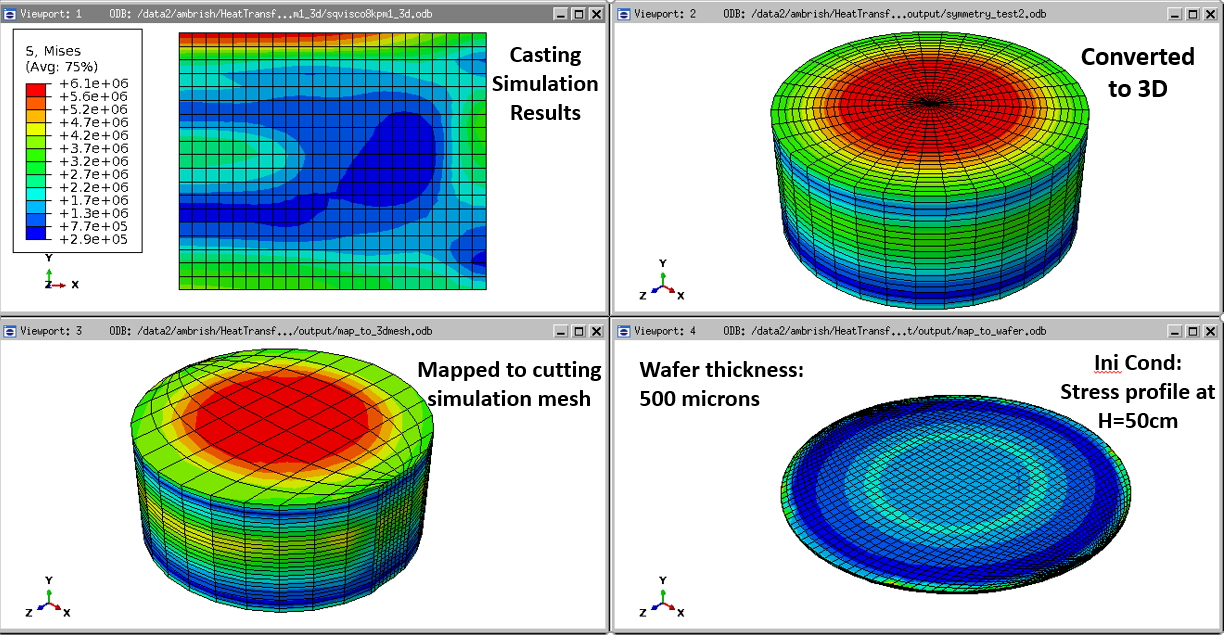
\includegraphics[width=6.0in]{mappings.PNG}
        \captionof{figure}{}.
        \label{fig:mappings}
 \end{minipage}


\begin{minipage}[c]{\textwidth}
\centering
        \captionsetup{type=figure}
        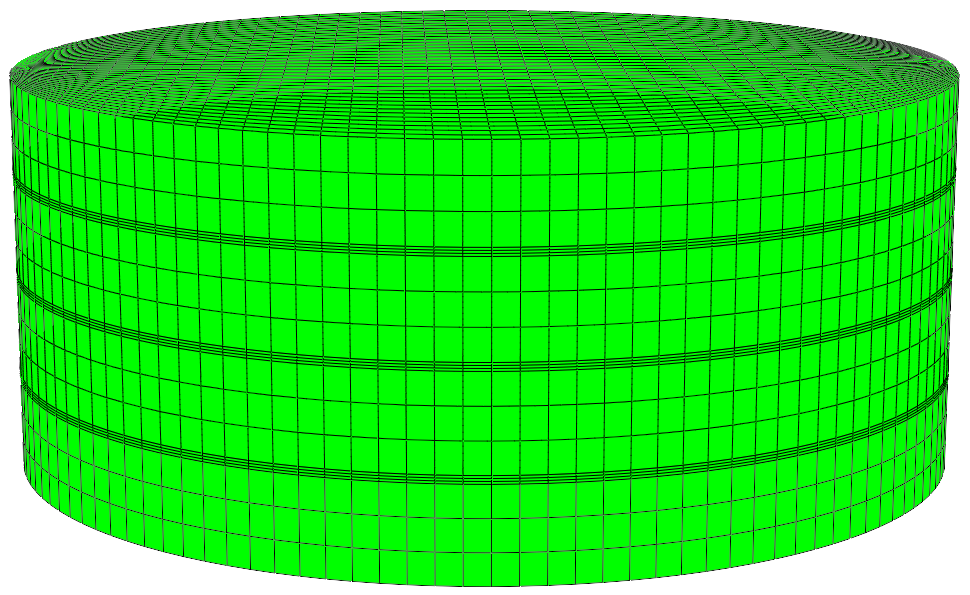
\includegraphics[width=2.0in]{wire-saw-mesh.PNG}
        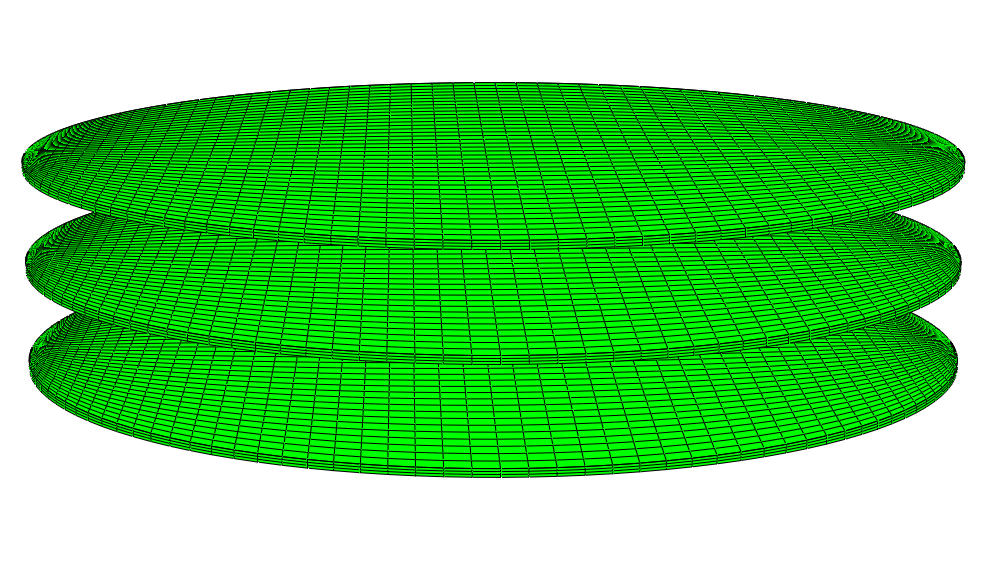
\includegraphics[width=2.0in]{wafer-kerf2.PNG}
        \captionof{figure}{}.
        \label{fig:model_change}
 \end{minipage}

%The volume where wire sawing simulation was done was 1000 micron thick sections at heights: 26.25,  52.5 & 79.75 mm, as shown in Figure \ref{fig:model_change}. These sections were 1000 micron thick because the wafer formed and the layers removed are both 500 micron as shown in Fig \ref{fig:cutting}. 

\begin{minipage}[c]{\textwidth}
\centering
         \captionsetup{type=figure}
        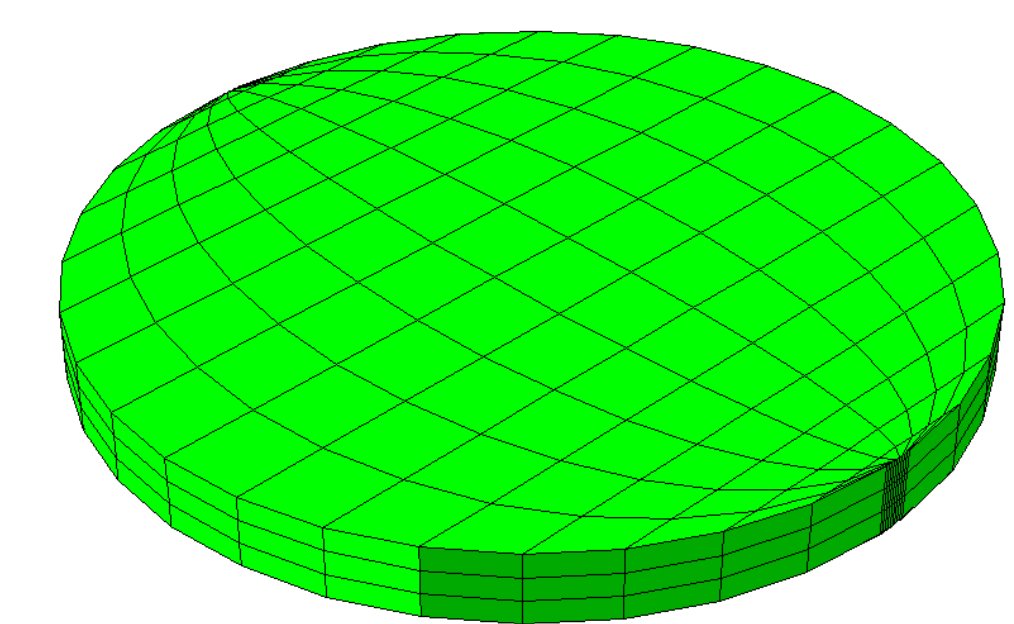
\includegraphics[width=2.0in]{cutting1.PNG}
        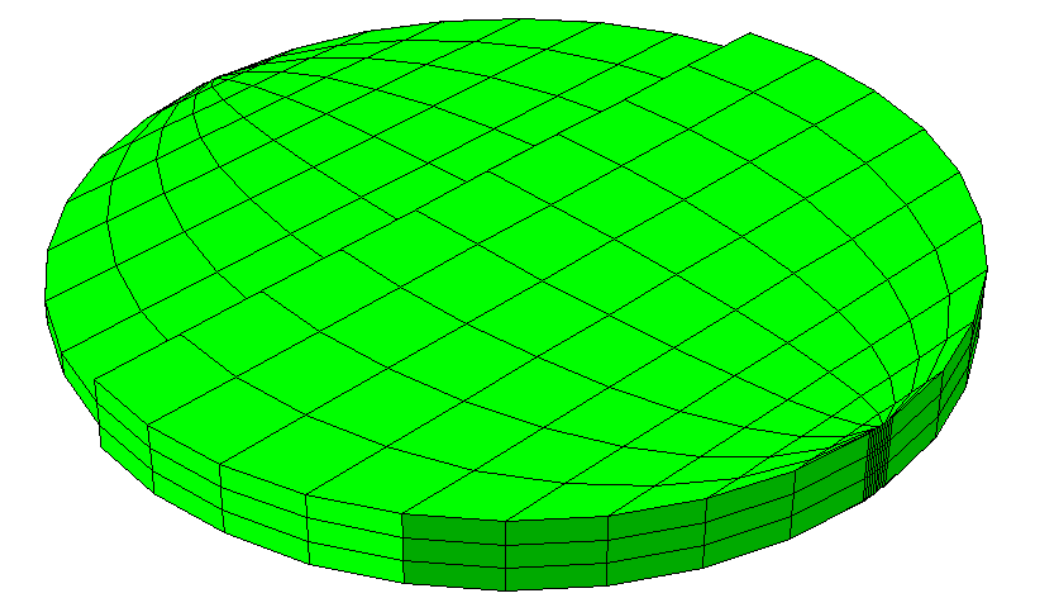
\includegraphics[width=2.0in]{cutting2.PNG}
        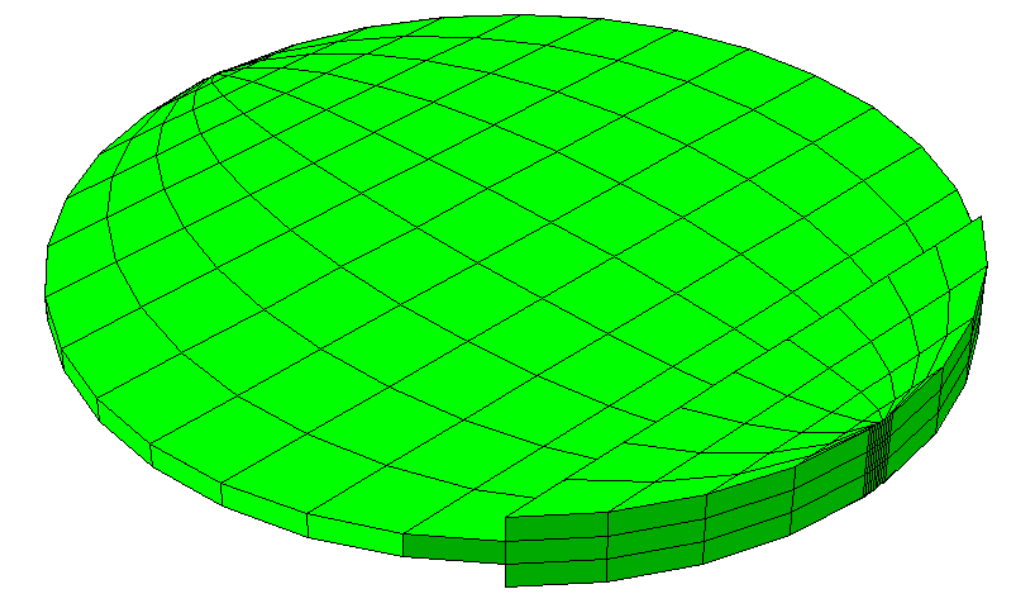
\includegraphics[width=2.0in]{cutting3.PNG}
        \captionof{figure}{}.
        \label{fig:cutting}
 \end{minipage}



%======================================================================
\chapter{Results}
%======================================================================

\section{Casting}

\subsection{Thermal Simulation}

\subsection{Stress Simulation}


\section{Wire Sawing}

\subsection{Thermal Simulation}

\subsection{Stress Simulation}


%% This file is setup to use a bibtex file sample.bib and uses the
%% plain style.  Other styles may be used depending on the conventions
%% of your field of study.
%%
%%% Note: the bibliography must come before the appendices.
\bibliographystyle{plain}
\bibliography{references}

%% Use this to reset the appendix counter.  Note that the FoGS
%% requires that the word ``Appendices'' appear in the table of
%% contents either before each appendix lable or as a division
%% denoting the start of the appendices.  We take the latter option
%% here.  This is ensured by making the \texttt{appendicestoc} option
%% a default option to the UBC thesis class.

%%% If you only have one appendix, please uncomment the following line.
% \renewcommand{\appendicesname}{Appendix}
\appendix
\chapter{First Appendix}
Here you can have your appendices.  Note that if you only have a
single appendix, you should issue
\verb|\renewcommand{\appendicesname}{Appendix}| before calling
\verb|\appendix| to display the singular ``Appendix'' rather than the
default plural ``Appendices''.

\chapter{Second Appendix}
Here is the second appendix.

%% This changes the headings and chapter titles (no numbers for
%% example).
\backmatter

%% Indices come here if you have them.

\chapter*{Additional Information}
This chapter shows you how to include additional information in your
thesis, the removal of which will not affect the submission.  Such
material should be removed before the thesis is actually submitted.

First, the chapter is unnumbered and not included in the Table of
Contents.  Second, it is the last section of the thesis, so its
removal will not alter any of the page numbering etc. for the previous
sections.  Do not include any floats, however, as these will appear in
the initial lists.

The \texttt{ubcthesis} \LaTeX{} class has been designed to aid you in
producing a thesis that conforms to the requirements of The
University of British Columbia Faculty of Graduate Studies (FoGS).

Proper use of this class and sample is highly recommended---and should
produce a well formatted document that meets the FoGS requirement.
Notwithstanding, complex theses may require additional formatting that
may conflict with some of the requirements.  We therefore \emph{highly
  recommend} that you consult one of the FoGS staff for assistance and
an assessment of potential problems \emph{before} starting final
draft.

While we have attemped to address most of the thesis formatting
requirements in these files, they do not constitute an official set of
thesis requirements.  The official requirements are available at the
following section of the FoGS web site:
\begin{center}
  \begin{tabular}{|l|}
    \hline
    \url{http://www.grad.ubc.ca/current-students/dissertation-thesis-preparation}\\
    \hline
  \end{tabular}
\end{center}
We recommend that you review these instructions carefully.

\end{document}
\endinput
%%
%% End of file `ubcsample.tex'.
